\documentclass{beamer}

% Note to the reader: if you find the word “WTF” in this TeX source,
% this means that some part of TeX is absolutely not behaving as
% specified in its documentation. It is usually followed by the name
% of the guilty person. Any presence of such a word in this document
% would be a perfectly valid excuse to throw out all of TeX into the
% bin and start over with people who actually know how to program.

\usepackage[no-math]{fontspec}
\usepackage{etoolbox}
\usepackage{array, amsmath, amsthm, mathtools, stmaryrd}
\usepackage{amssymb} % In theory incompatible with MnSymbol…
\usepackage{MnSymbol}
\usepackage{mathdots}

\usepackage{epsfig}
\usepackage{textpos}

\usepackage{scrhack} % To avoid some warnings

\usepackage{xfrac}
\usepackage[super]{nth}
%\usepackage[xetex, colorlinks=true]{hyperref}
\usepackage{epigraph}

\usepackage{caption}
%\usepackage[labelformat=parens,labelsep=space]{subcaption}
\DeclareCaptionLabelSeparator{nbspace}{~}
\usepackage[labelformat=parens,labelsep=nbspace]{subcaption}
\captionsetup{belowskip=8pt}
%\makeatletter % I don’t know why, but it seems that the space after the label is not taken into account.
%\newcommand*{\subcaption@old}{}
%\let\subcaption@old=\subcaption
%\renewcommand*{\subcaption}[1]{\subcaption@old{~#1}}
%\newcommand\subcaption
%\makeatother

\usepackage{multicol}

%\usepackage{float}
%\floatstyle{plaintop}
%\newfloat{program}{tbp}{progs}[chapter]
%\floatname{program}{Program}

\usepackage{newfloat}
%\DeclareFloatingEnvironment[
%    fileext = prog,
%    listname = {List of Programs},
%    name = Program,
%    placement = tbp,  % h adds a lot of space and breaks the reading flow.
%    within = chapter
%]{program}

% \usepackage{tocloft}

% \newcommand\listprogramname{List of Programs}
% \newlistof[chapter]{program}{prog}{\listprogramname}
% \cftsetindents{program}{0em}{3em}

% \DeclareNewTOC[
%     type = program,
%     types = programs,
%     float,
%     floatpos = tbp,  % h adds a lot of space and breaks the reading flow.
%     name = Program,
%     listname = {List of Programs},
%     counterwithin = chapter,
%     %tocentryindent = 3em,
%     hang = 3em,
%     indent = 0em,
%     %tocentrystyle=
% ]{prog}

%\DeclareCaptionSubType{program}

% \renewcommand\cftloftitlefont{\thesischapterfont}

%\graphicspath{{figures/}}

\usepackage{xunicode}
\defaultfontfeatures{Ligatures = TeX, Numbers = OldStyle}
\setmainfont{Linux Libertine O}
\setmonofont[Scale = MatchLowercase]{DejaVu Sans Mono}
\newfontfamily\garamond{EB Garamond}
\defaultfontfeatures[\garamond]{Ligatures = TeX, Numbers = Lining}
\newfontfamily\freeserif{FreeSerif}
\defaultfontfeatures[\freeserif]{Ligatures = TeX, Numbers = Lining}
\newfontfamily\libertine{Linux Libertine O}
\defaultfontfeatures[\libertine]{Ligatures = TeX, Numbers = OldStyle}
\newfontfamily\stix{XITS Math}
\newfontfamily\maguntia{UnifrakturMaguntia}
\defaultfontfeatures[\libertine]{Ligatures = TeX, Numbers = OldStyle}
\renewcommand\mathfrak[1]{% WTF XeLaTeX? Not enough alphabet?! #NeverTrustKnuth
    \mbox{\maguntia{}#1}%
}

\newcommand\xmark{{\freeserif{}❌}}
\newcommand\cmark{{\freeserif{}✓}}

\newcommand\Coq{Coq}
\newcommand\OCaml{OCaml}
\newcommand\R{R}

\newcommand*\pname[2][]{\ifnempty{#1}{#1~}{}{#2}}

\newcommand*\fcmp{\mathbin{\text{\stix{}⨾}}}

\newcommand*\unnummeredsection[1]{%
    \section*{#1}%
    \addcontentsline{toc}{section}{#1}%
}
\newcommand*\unnummeredchapter[1]{%
    \chapter*{#1}%
    \addcontentsline{toc}{chapter}{#1}%
}
\newcommand*\unnummeredpart[1]{%
    \part*{#1}%
    \addcontentsline{toc}{part}{#1}%
}

% An implementation of \@ifnextchars (which should be in the core TeX distribution, but whatever).
% It takes several characters and check whether once of them directly follows.
% Thanks to http://tex.stackexchange.com/questions/320696/trying-to-understand-how-cdr-nil-works-in-relation-to-expandafter/320707
% Usage:
% - \@ifnextchars{chars}{ true branch }{ false branch }
\makeatletter
\newcommand\@ifnextchars[3]{%
    \if\relax\detokenize{#1}\relax
        \def\@ifnextchars@tmp{#3}%
    \else%
        \edef\@ifnextchars@tmp{%
            % \def\@ifnextchars@car{\@car#1\@nil}%
            % \def\@ifnextchars@cdr{\@cdr#1\@nil}%
            % \expandafter\expandafter\expandafter\@ifnextchars@aux\expandafter%
            %     \@ifnextchars@car\@ifnextchars@cdr{#2}{#3}%
            \noexpand\@ifnextchars@aux%
                {\unexpanded\expandafter{\@car#1\@nil}}
                {\unexpanded\expandafter{\@cdr#1\@nil}}
                \unexpanded{{#2}{#3}}%
        }%
    \fi
    \@ifnextchars@tmp% This ugly def serves as putting \@ifnextchar
                     % in the outermost context. Otherwise, it runs
                     % into conflict with the \fi token.
}
\newcommand\@ifnextchars@aux[4]{%
    \expandafter\@ifnextchar#1{%
        #3%
    }{%
        \@ifnextchars{#2}{#3}{#4}%
    }%
}
\makeatother

\makeatletter
\newcommand*\kuneSimboloKomenco{\normalfont\freeserif{}⌜}
\newcommand*\kuneSimboloFino{\normalfont\freeserif{}⌝}
\newcommand*\kune@koloro{Aluminium2}
\newcommand*\kune@komenco{%
    \hspace{-1pt}\makebox[1pt][l]{\textcolor{\kune@koloro}{\kuneSimboloKomenco{}}}%
}
\newcommand*\kune@fino{%
    \makebox[0pt][r]{\textcolor{\kune@koloro}{\kuneSimboloFino{}}}%
}
% \kune{text} groups a text.
% It prints symbols similar to parentheses, but for text.
\newcommand*\kune[1]{%
    \kune@komenco{}%
    #1%
    \nobreak%
    \hspace{1pt}%
    \nobreak%
    \kune@fino%
    % Dealing with the punctuation characters.
    \@ifnextchars{.,-—}{%
        \nobreak%
        \hspace{-1pt}%
    }{%
        \@ifnextchars{;?!:)’”}{%
            \nobreak%
        }{%
            % \@ifnextchar eats spaces: if no character is recognised, we add a space.
            \hspace{-1pt}
        }%
    }%
}
% For the rare cases in which \kune has to be used at
% the beginning of a quotation or a parenthesis,
% I also provide this alternative command.
\newcommand*\kunec[1]{%
    \hspace{1pt}\nobreak%
    \kune{#1}%
}
% \kunef{text} is a non-fragile variant of kune.
% It does not however perform look-ahead tweaks and might produce
% typographical oddities if used at the end of a sentence.
\newcommand*\kunef[1]{%
    % \protect{\kune{#1}}%
    \kune@komenco{}%
    #1%
    \nobreak%
    \hspace{1pt}%
    \kune@fino%
    \hspace{-1pt}%
}
\makeatother

% Commands for abbreviations.
\newcommand*\mallongigo[2][]{%
    \hyperlink{mallongigo:#2}{\ifempty{#1}{#2}{#1}}%
}
\newcommand*\mallongigi[2]{%
    \hypertarget{mallongigo:#1}{#2} (\mallongigo{#1})%
}
% Usage:
%   - \mallongigi{AST}{abstract syntax tree}
% This defines some hyperlinks, which then allow to do:
%   - \mallongigo{AST}.
%   - \mallongigo[ASTs]{AST}.
% Note that the abbreviation (“AST” in the example) should be usable as a target label.

\newcommand\quotec[1]{\textup{[#1]}}
\newcommand*\elide{\quotec{…}}

\newcommand\ifempty[3]{\expandafter\ifstrempty{#1}{#2}{#3}}
\newcommand\ifnempty[2]{\expandafter\ifstrempty{#1}{}{#2}}
\newcommand\defaultempty[2]{\expandafter\ifstrempty{#1}{#2}{#1}}
\newcommand\ignore[1]{}

\newcommand*\mathsc[1]{\mathrm{\textsc{#1}}}

\newcommand*\none{\mbox{\coqinline|None|}}
\newcommand*\some[1]{\mbox{\coqinline|Some|}\funu{#1}}
\newcommand*\option[1]{\mathit{option}\ifnempty{#1}{\ #1}}
% \newcommand*\option[1]{{#1}^?}
\newcommand*\struct{\mathit{struct}}

\newcommand*\Prog{\ensuremath{\mathit{Prog}}}
\newcommand*\Val{\ensuremath{\mathit{Val}}}
\newcommand*\ALoc{\ensuremath{\mathit{ALoc}}}
\newcommand*\Env{\ensuremath{\mathit{Env}}}
\newcommand*\env{\ensuremath{\mathit{env}}}
\newcommand*\State{\ensuremath{\mathit{State}}}
\newcommand*\Store{\ensuremath{\mathit{Store}}}
\newcommand*\Heap{\ensuremath{\mathit{Heap}}}
\newcommand*\Var{\ensuremath{\mathit{Var}}}
\newcommand*\LVar{\ensuremath{\mathcal{X}}}
\newcommand*\PP{\ensuremath{\mathit{PP}}} % Program point
\newcommand*\Field{\ensuremath{\mathit{Field}}}
\newcommand*\Trace{\ensuremath{\mathit{Trace}}}
\newcommand*\Dep{\ensuremath{\mathit{Dep}}}
\newcommand*\Stor{\ensuremath{\mathit{Store}}}
\newcommand*\Source{\ensuremath{\mathit{Source}}}
\newcommand*\Mut{\ensuremath{\mathit{Mut}}}
\newcommand*\Bool{\ensuremath{\mathit{Bool}}}
\newcommand*\Envf{\ensuremath{\mathit{Env}_f}}
\newcommand*\fNames{\ensuremath{\mathit{Names}}}
\newcommand*\stat{\ensuremath{\mathit{stat}}}

\newcommand*\freshHeap{\ensuremath{\mathit{fresh}\funu}}

\newcommand*\Stat{\ensuremath{\mathit{Stat}}}
\newcommand*\Expr{\ensuremath{\mathit{Expr}}}

\newcommand*\undefv{\ensuremath{\mathit{undef}}}

\makeatletter % There may be a simpler way to do this.
\newcommand*\@absstarnothing[1]{\ensuremath{\mathrel{#1^\sharp}}}
\newcommand*\@absnostarnothing[1]{\ensuremath{{#1^\sharp}}}
\def\@absstarbrack#1[#2]{\ensuremath{\mathrel{#1[#2]^\sharp}}}
\def\@absnostarbrack#1[#2]{\ensuremath{{#1[#2]^\sharp}}}
\newcommand*\@absstarnounder[1]{%
    \@ifnextchar[{\@absstarbrack{#1}}{\@absstarnothing{#1}}}
\newcommand*\@absnostarnounder[1]{%
    \@ifnextchar[{\@absnostarbrack{#1}}{\@absnostarnothing{#1}}}
\def\@absstarunder#1_#2{\ensuremath{\mathrel{#1_{#2}^\sharp}}}
\def\@absnostarunder#1_#2{\ensuremath{{#1_{#2}^\sharp}}}
\newcommand*\@absstarchoice[1]{%
    \@ifnextchar_{\@absstarunder{#1}}{\@absstarnounder{#1}}}
\newcommand*\@absnostarchoice[1]{%
    \@ifnextchar_{\@absnostarunder{#1}}{\@absnostarnounder{#1}}}
\newcommand*\abs{\@ifstar\@absstarchoice\@absnostarchoice}
\makeatother
\newcommand*\bigabs[1]{\mathop{\abs*{{#1}}}}

% Lambda-calculus constructions
\newcommand*\lcfun[2]{\ensuremath{\lambda #1.\ #2}}
\newcommand*\lcapp[2]{\ensuremath{@\ifnempty{#1}{\,#1}\ifnempty{#2}{\,#2}}}
\newcommand*\lcappx[2][]{\ensuremath{@_1\ifnempty{#1}{\,#1}\,#2}}
\makeatletter
\newcommand*\lcappxx@final[2]{\ensuremath{@_2\ifnempty{#1}{\,#1}\ifnempty{#2}{\,#2}}}
\def\lcappxx@u#1[#2]{\lcappxx@final{#1}{#2}}
\newcommand*\lcappxx@d[1][]{\@ifnextchar[{\lcappxx@u{#1}}{\lcappxx@final{#1}{}}}
\newcommand*\lcappxx{\lcappxx@d}
\makeatother

\newcommand*\pbshole{{\cdot}}

\newcommand*\p[2]{#1 + #2}
\newcommand*\px[1]{\pbshole{} +_1 #1}
\newcommand*\pxx[0]{\pbshole{} +_2 \pbshole{}}

\newcommand*\gr[2]{#1 > #2}
\newcommand*\grx[1]{\pbshole{} >_1 #1}
\newcommand*\grxx[0]{\pbshole{} >_2 \pbshole{}}

\newcommand*\op[3]{#2 #1 #3}
\newcommand*\opx[2]{\pbshole{} #1_1 #2}
\newcommand*\opxx[1]{\pbshole{} #1_2 \pbshole{}}

\newcommand*\snot[1]{\neg #1}
\newcommand*\snotx{\neg_1 \pbshole{}}

\newcommand*\eq[2]{#1 = #2}
\newcommand*\eqx[1]{\pbshole{} =_1 #1}
\newcommand*\eqxx[0]{\pbshole{} =_2 \pbshole{}}

\newcommand*\property[2]{#1\jsid{.#2}}
\newcommand*\propertyx[1]{\jsid{.#1}}

\newcommand*\hasfield[2]{\jsid{#1}\,\mathit{in}\,{#2}}
\newcommand*\hasfieldx[1]{\jsid{#1}\,\mathit{in}_1 \pbshole{}}

\newcommand*\rfield[2]{#1\jsid{.#2}}
\newcommand*\rfieldx[1]{\jsid{.#1}}

\newcommand*\arobase{@}

\newcommand*\lambdaexp[2]{\lambda \jsid{#1} . {#2}}
\newcommand*\funapp[2]{{#1}\funu{#2}}
\newcommand*\funappx[1]{\arobase_1\funu{#1}}
\newcommand*\funappxx{\arobase_2}
\newcommand*\funappxxx{\arobase_3}

\newcommand*\asn[2]{\jsid{#1}\ {:=}\ #2}
\newcommand*\asnx[1]{\jsid{#1}\ {:=_1}\ \pbshole{}}
\newcommand*\rasn[2]{#1\ {:=}\ #2}

\newcommand*\asnp[3]{#1\jsid{.#2}\ {:=}\ #3}
\newcommand*\asnpx[2]{\jsid{.#1}\ {:=_1}\ #2}
\newcommand*\asnpxx[1]{\jsid{.#1}\ {:=_2}\ \pbshole{}}

\newcommand*\delete[2]{\mathit{delete}\ #1\jsid{.#2}}
\newcommand*\deletex[1]{\mathit{delete}_1\ \jsid{.#1}}

\newcommand*\seq[2]{\mathit{seq}\ #1\ #2}
\newcommand*\seqx[1]{\mathit{seq}_1\ #1}
\newcommand*\seqxx{\mathit{seq}_2}
\newcommand*\rseq[2]{#1 ; #2}

\newcommand*\iname{\mathit{if}}

\newcommand*\sif[3]{\iname\ifnempty{#1#2#3}{\,#1\,#2\ifnempty{#3}{\,#3}}}
\newcommand*\sifx[2]{\iname_1\ifnempty{#1#2}{\,#1\ifnempty{#2}{\,#2}}}

\newcommand*\lreturn[1]{\mathit{return}\ifnempty{#1}{\,#1}}
\newcommand*\lreturnx{\mathit{return}_1 \pbshole{}}

\newcommand*\lrun[1]{\mathit{run}\ifnempty{#1}{\,#1}}
\newcommand*\lrunx{\mathit{run}_1 \pbshole{}}

\newcommand*\wname{\mathit{while}}
\newcommand*\wxname{\wname_1}
\newcommand*\wxxname{\wname_2}

\newcommand*\while[2]{\wname\ifnempty{#1}{\,#1}\ifnempty{#2}{\,#2}}
\newcommand*\whilex[2]{\wxname\ifnempty{#1}{\,#1}\ifnempty{#2}{\,#2}}
\newcommand*\whilexx[2]{\wxxname\ifnempty{#1}{\,#1}\ifnempty{#2}{\,#2}}

\newcommand*\throw{\mathit{throw}}

\newcommand*\sskip{\mathit{skip}}

\usepackage{tikz}

\usetikzlibrary{trees, arrows, shapes, automata, petri}
\usetikzlibrary{fit, calc, decorations}
\usetikzlibrary{decorations.pathreplacing}
\usetikzlibrary{decorations.pathmorphing}
\usetikzlibrary{positioning}
\usetikzlibrary{shadings, fadings, patterns}
%\usepackage{pgfbaselayers}
\pgfdeclarelayer{background}
\pgfdeclarelayer{foreground}
\pgfsetlayers{background,main,foreground}

\newcommand*\myimg[2][2cm]{%
    \begin{center}%
        \includegraphics[height=#1]{imgs/#2}
    \end{center}%
}

\makeatletter
\newcommand\hiddenbox@basic[4]{%
    \parbox[0cm]{\textwidth}{%
        \only<#1>{%
            \vspace{#2}%
            \begin{block}{#3}%
                #4%
            \end{block}%
        }%
    }%
}
\def\hiddenbox@eattitle#1#2[#3]{%
    \hiddenbox@basic{#1}{#2}{#3}%
}
\def\hiddenbox@eatdim#1[#2]{%
    \@ifnextchar[{\hiddenbox@eattitle{#1}{#2}}{\hiddenbox@eattitle{#1}{#2}[]}%
}
\def\hiddenbox@eatonly<#1>{%
    \@ifnextchar[{\hiddenbox@eatdim{#1}}{\hiddenbox@eatdim{#1}[0cm]}%
}
\newcommand\hiddenbox{%
    \@ifnextchar<{\hiddenbox@eatonly}{\hiddenbox@eatonly<1->}%
}
\newcommand*\hiddenimage@basic[4]{%
    \parbox[0cm]{\textwidth}{%
        \only<#1>{%
            \vspace{#2}%
            \myimg[#3]{#4}%
        }%
    }%
}
\def\hiddenimage@eatsize#1#2[#3]{%
    \hiddenimage@basic{#1}{#2}{#3}%
}
\def\hiddenimage@eatdim#1[#2]{%
    \@ifnextchar[{\hiddenimage@eatsize{#1}{#2}}{\hiddenimage@eatsize{#1}{#2}[2cm]}%
}
\def\hiddenimage@eatonly<#1>{%
    \@ifnextchar[{\hiddenimage@eatdim{#1}}{\hiddenimage@eatdim{#1}[0cm]}%
}
\newcommand*\hiddenimage{%
    \@ifnextchar<{\hiddenimage@eatonly}{\hiddenimage@eatonly<1->}%
}
\makeatother

\tikzset{
	location/.style = {
		draw = Aluminium6,
		rectangle,
		rounded corners = 2pt,
		text centered,
		minimum height = 5mm,
		minimum width = 10mm,
		top color = white,
		bottom color = Aluminium1
	},
	new location/.style = {
		location,
		top color = LightOrange,
		bottom color = Orange
	},
	orange location/.style = {
		location,
		top color = Aluminium1,
		bottom color = LightOrange
	}
}

\tikzset{
	code node/.style = {
		rectangle,
		text centered,
		rounded corners = 3pt,
		minimum height = 1cm,
		minimum width = 2cm,
		top color = Aluminium1,
		bottom color = Aluminium2,
		draw = Aluminium3
	},
	green code/.style = {
		code node,
		bottom color = Chameleon,
		draw = Chameleon
	},
	orange code/.style = {
		code node,
		bottom color = LightOrange,
		draw = orange
	},
	red code/.style = {
		code node,
		bottom color = LightScarletRed,
		draw = ScarletRed
	},
	yellow code/.style = {
		code node,
		top color = white,
		bottom color = LightButter,
		draw = DarkButter
	}
}

\tikzset{
  locnode base/.style = {
    rectangle,
    rounded corners = 2pt,
    text centered,
    minimum height = 5mm,
    minimum width = 10mm,
    bottom color = white,
    top color = white
  },
  locnode grey/.style = {
    locnode base,
    draw = Aluminium6,
    bottom color = Aluminium2
  },
  locnode/.style = {
    locnode grey
  },
  locnode orange/.style = {
    locnode base,
    draw = DarkOrange,
    bottom color = Orange
  },
  locnode green/.style = {
    locnode base,
    draw = DarkChameleon,
    bottom color = Chameleon
  },
  locnode red/.style = {
    locnode base,
    draw = DarkScarletRed,
    bottom color = ScarletRed
  },
  locnode plum/.style = {
    locnode base,
    draw = DarkPlum,
    bottom color = LightPlum
  },
  locnode blue/.style = {
    locnode base,
    draw = DarkSkyBlue,
    bottom color = LightSkyBlue
  },
  locnode brown/.style = {
    locnode base,
    draw = DarkChocolate,
    bottom color = LightChocolate
  },
  locnode yellow/.style = {
    locnode base,
    draw = DarkButter,
    bottom color = Butter
  },
  abstraction source/.style = {
    locnode green
  },
  abstraction proposition/.style = {
    locnode plum
  },
  abstraction trace/.style = {
    locnode brown
  },
}

\newcommand\partandfile[4][]{
    \node [yellow code, #1] (#2) {\begin{tabular}{c}#3\end{tabular}} ;
    \node [code node, below = 0pt of #2] (#2file) {\tt{}\begin{tabular}{c}#4\end{tabular}} ;
}

\newcommand*\derivationAbove[2][1cm]{
    \begin{pgfonlayer}{background}
        \begin{scope}[decoration = {zigzag, segment length = 6.45mm, amplitude = 1mm}]
        \fill [draw = DarkSkyBlue, top color = LightSkyBlue, bottom color = LightSkyBlue!0]
            (#2.north west) -- ($(#2.north west) + (-#1, #1)$)
            decorate { -- ($(#2.north east) + (#1, #1)$)}
            -- (#2.north east) -- cycle ;
        \end{scope}
        \draw [white, very thick] (#2.north east) -- (#2.north west) ;
    \end{pgfonlayer}
}

\tikzset{
    blob/.style = {
        %ellipse,
        %decoration = {snake, aspect = 0, segment length = 4mm, amplitude = .4mm}, decorate,
        star, star points = 6, rounded corners = 1.5mm,
        %cloud, cloud puffs = 3, cloud puff arc = 200, cloud ignores aspect,
        %decoration={random steps, segment length = 2mm}, decorate,
        %rounded corners = 1mm,
        minimum width = 8mm, minimum height = 1cm,
        draw = Plum, fill = Plum!10
    }
}

\newcommand*\single[3][]{
    \node [#1, minimum width = 0pt, minimum height = 0pt] (#2) {} ;
    \node [at = (#2)] {\(\bullet\)} ;
    \node [at = (#2), above] {#3}
}
\newcommand*\singlec[4][]{
    \node [#1, minimum width = 0pt, minimum height = 0pt] (#3) {} ;
    \node [#2, at = (#3)] {\(\bullet\)} ;
    \node [#2, at = (#3), above] {#4}
}


%\theoremstyle{plain}
%\newtheorem{theorem}{Theorem}[chapter]
%\newtheorem{lemma}[theorem]{Lemma}
%\newtheorem{proposition}[theorem]{Proposition}
%\newtheorem{corollary}[theorem]{Corollary}
%\newtheorem{conjecture}[theorem]{Conjecture}
%% \newtheorem{hypothesis}{Hypothesis}[chapter]
%\newtheorem{hypothesis}[theorem]{Hypothesis}

%\theoremstyle{definition}
%\newtheorem{definition}{Definition}[chapter]


\newenvironment{ex}[1][Example.]{\begin{trivlist}
\item[\hskip \labelsep {\bfseries #1}]}{\end{trivlist}}

\newcommand*\sepstar{%
	\mathrel{\ooalign{%
			\hss$\sqcup$\hss\cr%
            \hss\raisebox{1pt}{\(\star\)}\hss\cr%
	}}
}

\newcommand*\dom[1]{\textrm{dom}(#1)}
\newcommand*\codom{\mathit{codom}\funu}
\newcommand*\interface{\mathit{itf}\funu}
\newcommand*\spec{\mathit{spec}\funu}

\newcommand*\reduce[1][]{\overset{#1}{\longrightarrow}}
\newcommand*\reducebot[1][]{\expandafter\ifstrempty{#1}{\Downarrow}{\Botarrow_{#1}}}
\newcommand*\abort[1]{\mathbf{abort}\ifnempty{#1}{\,#1}}
\newcommand*\intercept[2]{\mathbf{intercept}\ifnempty{#1}{_{#1}}\ifnempty{#2}{\,#2}}
%\newcommand*\normal[2]{\mathit{normal}\,#1\,#2}

\newcommand*\ToPrimitive{\mathit{ToPrimitive}}
\newcommand*\ToString{\mathit{ToString}}
\newcommand*\ToBoolean{\mathit{ToBoolean}}

\newcommand*\javascript{\textsc{Ja\-va\-Script}}
\newcommand*\jsfuck{\textsc{JSFuck}}
\newcommand*\ecmascript[1][]{{ECMA\-Script}\ifnempty{#1}{~#1}}
\newcommand*\whilel{\textsc{While}}
\newcommand*\coqn{\textsc{Coq}}
\newcommand*\camln{\textsc{OCaml}}
\newcommand*\camll{\textsc{Caml Light}}
\newcommand*\smlc{\textsc{Standard ML}}
\newcommand*\Cn[1][]{\textsc{C#1}}
\newcommand*\Cminor{\Cn[\(\sharp\)minor]{}}
\newcommand*\haskell{\textsc{Has\-kell}}
\newcommand*\lambdajs{\mbox{\(\lambda_\text{JS}\)}}
\newcommand*\Kn{\mbox{\(\mathbb{K}\)}}
\newcommand*\kjs{\textsc{KJS}}
\newcommand*\Isabelle{\textsc{Isabelle/Hol}}
\newcommand*\CompCert{\textsc{Comp\-Cert}}
\newcommand*\Java{\textsc{Java}}
\newcommand*\Shell{\textsc{Shell}}
\newcommand*\Lisp{\textsc{Lisp}}
\newcommand*\Scala{\textsc{Scala}}
\newcommand*\Python{\textsc{Python}}
\newcommand*\llvm{\textsc{LLVM}}

\newcommand*\jscert{\textsc{JSCert}}
\newcommand*\jsref{\textsc{JSRef}}
\newcommand*\jsexplain{\textsc{JSExplain}}

\newcommand*\etal{\emph{et al.}}

\newcommand*\forin{\jsinline|for|-\jsinline|in|}
\newcommand*\trycatchfinally{\jsinline|try|-\jsinline|catch|-\jsinline|finally|}

\newcommand*\Mozilla{\textsc{Mozilla}}
\newcommand*\Firefox{\textsc{Mozilla Firefox}}
\newcommand*\Chromium{\textsc{Chromium}}

\usepackage{todonotes}
\newcommand\as[1]{\todo[color=green!40,size=\scriptsize,caption={}]{#1}}
\newcommand\asi[1]{\todo[inline,caption={},color=green!40]{#1}}
\newcommand\mb[1]{\todo[color=LightPlum!80,size=\scriptsize]{#1}}
\newcommand\mbi[1]{\todo[color=LightPlum!80,inline]{#1}}
\newcommand\tj[1]{\todo[color=yellow!30,size=\scriptsize]{#1}}
\newcommand\tji[1]{\todo[color=yellow!30,inline]{#1}}

\newcommand*\owhile{\textsc{O’While}}

\newcommand*\qqquad{\quad\qquad}
\newcommand*\qqqquad{\quad\qqquad}

\newenvironment{changemargin}[2]
    {\list{}{\rightmargin#2\leftmargin#1}\item[]}
    {\endlist}

\newenvironment{widemargin}
    {\begin{changemargin}{-2cm}{-2cm}}
    {\end{changemargin}}

\usepackage{longtable}

\newenvironment{codemath}
    {
\begin{widemargin}
    \begin{longtable}{>{\(}l<{\)}}
            \endfirsthead
            \endhead
            \endfoot
            \endlastfoot
    }
    {
    \end{longtable}\hfill\ 
\end{widemargin}
    }

\xdef\isgreyexpr{n}
\newcommand*\grey[1]{%
	\def\greyargument{#1}%
    \expandafter\ifstrequal{\isgreyexpr}{n}{
		\xdef\isgreyexpr{y}%
		\textcolor{Aluminium4}{\greyargument}\,%
		\xdef\isgreyexpr{n}%
	}{\greyargument}%
}

\xdef\isinunderlinejsexpr{n}
\newcommand*\jsexpr[2][Aluminium3]{%
    \expandafter\ifstrequal{\isgreyexpr}{n}%
    {\textcolor{#1}}{}{%
    \def\jsexprargument{\expandafter\ifstrequal{\isgreyexpr}{n}{\textcolor{black}}{}{#2}}%
        \expandafter\ifstrequal{\isinunderlinejsexpr}{n}{
			\xdef\isinunderlinejsexpr{y}%
			\underline\jsexprargument%
			\xdef\isinunderlinejsexpr{n}%
		}{\jsexprargument}%
    }}

\newcommand*\jsexprl[3][Aluminium3]{%
	\jsexpr[#1]{\left[#3\right]^{#2}}%
}
\newcommand*\ifthenabove[1]{%
	\expandafter\ifstrempty{#1}{}{^{#1}}%
}

\newcommand*\aloc[2]{#1^{#2}}
\newcommand*\loc{\ensuremath{\ell}}
\newcommand*\eloc{\ensuremath{\ell_e}}
\newcommand*\cloc{\ensuremath{\ell_c}}
\newcommand*\state{S}
\newcommand*\clos[3]{%
    \ifempty{#3}%
    {\lambdaexp{#1}{#2}}%
    {\mpar{#3, \lambdaexp{#1}{#2}}}%
}

\newcommand*\formapprox{\ensuremath{\preccurlyeq}}

\newcommand*\jsid[2][]{{\textup{\texttt{\small #2}}\ifthenabove{#1}}}

\def\nsem{\,;_{\scalebox{.5}1}}
\def\nseq{\,=_{\scalebox{.5}1}}
\def\nseqq{\,=_{\scalebox{.5}2}}
\def\nsop{\;\texttt{op}_{\scalebox{.5}1}\;}
\def\nsopp{\;\texttt{op}_{\scalebox{.5}2}\;}
\def\nsdot{\,._{\scalebox{.5}1}}

\newcommand*\seqq[2]{\jsexpr{#1 \nsem #2}}

\usepackage{mathpartir}

% From http://tex.stackexchange.com/questions/99316/symbol-for-external-links
\newcommand*\ExternalLink[2][]{%
    \tikz[x = 1.2ex, y = 1.2ex, baseline = -0.05ex]{% 
        \begin{scope}[x = 1ex, y = 1ex]
            \clip (-0.1, -0.1) 
                --++ (-0, 1.2) 
                --++ (0.6, 0) 
                --++ (0, -0.6) 
                --++ (0.6, 0) 
                --++ (0, -1);
            \path [draw = #2, line width = 0.5, rounded corners = 0.5] (0, 0) rectangle (1, 1) ;
        \end{scope}
        \path [draw = #2, line width = 0.5] (0.5, 0.5) -- (1, 1) ;
        \path [draw = #2, line width = 0.5] (0.6, 1) -- (1, 1) -- (1, 0.6) ;
        \begin{scope}[xshift = 0.6ex, yshift = 0.6ex]
            \node (0, 0) {#1{\XeTeXLinkBox{\phantom{\rule{1.3ex}{1.3ex}}}}} ;
        \end{scope}
    }
}

\newcommand*\urllink[2][DarkPlum]{%
    \ExternalLink[\href{#2}]{#1}%
}

\newcommand*\companionlink[2][DarkPlum]{%
    \urllink[#1]{http://people.irisa.fr/Martin.Bodin/doktorigxo/#2}%
}

\usepackage[langlinenos,cache,newfloat]{minted}

\setminted{encoding=utf8}

\makeatletter
\newcommand{\minted@def@optcl@switch@simple}[2]{%
  \define@booleankey{minted@opt@g}{#1}%
    {\minted@addto@optlistcl{\minted@optlistcl@g}{#2}%
      \@namedef{minted@opt@g:#1}{true}}
    {\minted@addto@optlistcl{\minted@optlistcl@g}{}%
      \@namedef{minted@opt@g:#1}{false}}
  \define@booleankey{minted@opt@g@i}{#1}%
    {\minted@addto@optlistcl{\minted@optlistcl@g@i}{#2}%
      \@namedef{minted@opt@g@i:#1}{true}}
    {\minted@addto@optlistcl{\minted@optlistcl@g@i}{}%
      \@namedef{minted@opt@g@i:#1}{false}}
  \define@booleankey{minted@opt@lang}{#1}%
    {\minted@addto@optlistcl@lang{minted@optlistcl@lang\minted@lang}{#2}%
      \@namedef{minted@opt@lang\minted@lang:#1}{true}}
    {\minted@addto@optlistcl@lang{minted@optlistcl@lang\minted@lang}{}%
      \@namedef{minted@opt@lang\minted@lang:#1}{false}}
  \define@booleankey{minted@opt@lang@i}{#1}%
    {\minted@addto@optlistcl@lang{minted@optlistcl@lang\minted@lang @i}{#2}%
      \@namedef{minted@opt@lang\minted@lang @i:#1}{true}}
    {\minted@addto@optlistcl@lang{minted@optlistcl@lang\minted@lang @i}{}%
      \@namedef{minted@opt@lang\minted@lang @i:#1}{false}}
  \define@booleankey{minted@opt@cmd}{#1}%
      {\minted@addto@optlistcl{\minted@optlistcl@cmd}{#2}%
        \@namedef{minted@opt@cmd:#1}{true}}
      {\minted@addto@optlistcl{\minted@optlistcl@cmd}{}%
        \@namedef{minted@opt@cmd:#1}{false}}
}
\minted@def@optcl@switch@simple{kwrename}{-F kwrenamefilter}
\makeatother

\usepackage{tcolorbox}

\tcbuselibrary{minted, skins}

\tcbset{programbox/.style = {
        enhanced,
        colback = LightPlum!10,
        colframe = DarkPlum,
        left = 1mm,
        listing only,
        listing engine = minted
    }
}

% Definition of programming languages used in the document.
\makeatletter
\newcommand\makenewlistings@aux[2]{
    \expandafter\newtcblisting{#2code}[1][]{
        programbox,
        listing only,
        minted language = #1,
        minted options= {
            kwrename,
            linenos = true,
            fontsize = \small,
            escapeinside = @@,
            ##1}
    }
    \expandafter\newtcblisting{#2codelink}[2][]{
        programbox,
        listing only,
        minted language = #1,
        minted options= {
            kwrename,
            linenos = true,
            fontsize = \small,
            escapeinside = @@,
            ##1},
        overlay = {
                \begin{scope}[shift={([xshift=-1em, yshift=-1em]frame.north east)}]
                    \node (0, 0) {##2} ;
                \end{scope}
            }
    }
    \newmintinline[#2inline]{#1}{
        breaklines = true,
        escapeinside = @@,
        breakbytoken = true
    }
    \newmintinline[#2inlinenoescape]{#1}{
        breaklines = true,
        breakbytoken = true
    }
}
\newcommand\makenewlistings[2][]{
    \expandafter\makenewlistings@aux{\defaultempty{#1}{#2}}{#2}
}
\makeatother

% Fixing bug between minted and polyglossia.
\BeforeBeginEnvironment{minted}{\begin{english}}
\AfterEndEnvironment{minted}{\end{english}}

\makenewlistings{text}
\makenewlistings[extcoq]{coq}
\makenewlistings[ocaml]{caml}
\makenewlistings{js}
\makenewlistings[extk]{k}
\makenewlistings{pascal}
\makenewlistings{c}
\makenewlistings{R}

\usepackage{newunicodechar}
\newunicodechar{⊥}{$\bot$}
\newunicodechar{⊑}{$\sqsubseteq$}
\newunicodechar{⊤}{$\top$}
\newunicodechar{∨}{$\lor$}
\newunicodechar{∧}{$\land$}
\newunicodechar{∧}{$\land$}
\newunicodechar{⇒}{$\Rightarrow$}
\newunicodechar{∀}{$\forall$}
\newunicodechar{∃}{$\exists$}
\newunicodechar{→}{$\rightarrow$}
\newunicodechar{¬}{$\neg$}
\newunicodechar{↔}{$\leftrightarrow$}
%\usepackage{unicode-math}
%\setmainfont{TeX Gyre Termes}
%\setmathfont{TeX Gyre Termes Math}


%\newcommand*\jscom[1]{\textrm{\textcolor{DarkChameleon}{#1}}}%\lstinline|#1|}}
\newcommand*\jscom{\mintinline{js}}

\newcommand*\jsif[3]{\jsexpr{\jscom{if}\ #1\ \jscom{then}\ #2\ \jscom{else}\ #3}}
\newcommand*\jsiff[3]{\jsexpr{\jscom{if1}(#1,#2,#3)}}

\newcommand*\jswhile[2]{\jsexpr{\jscom{while}\ #1\ \jscom{do}\ #2}}
\newcommand*\jswhilee[3]{\jsexpr{\jscom{while1}(#1,#2,#3)}}
\newcommand*\jswhileee[3]{\jsexpr{\jscom{while2}(#1,#2,#3)}}

\newcommand*\jsass[3][]{\jsexpr{\jsid{#2}\ifthenabove{#1}\ \jscom{=}\ #3}}
\newcommand*\jsasss[3][]{\jsexpr{\jsid{#2}\ifthenabove{#1} \nseq #3}}

\newcommand*\jsdelete[3][]{\jsexpr{\jscom{delete}\ {#2}\ifthenabove{#1}\jscom{.}\jsid{#3}}}
\newcommand*\jsdeletee[3][]{\jsexpr{\jscom{delete1}\ifthenabove{#1}\ #2\jscom{.}\jsid{#3}}}

\newcommand*\jsfieldass[4][]{\jsexpr{#2.\jsid{#3}\ifthenabove{#1}\ \jscom{=}\ #4}}
\newcommand*\jsfieldasss[3]{\jsexpr{#1.\jsid{#2} \nseq #3}}
\newcommand*\jsfieldassss[3]{\jsexpr{#1.\jsid{#2} \nseqq #3}}

\newcommand*\jsop[2]{\jsexpr{#1\ \texttt{op}\ #2}}
\newcommand*\jsopp[2]{\jsexpr{#1 \nsop #2}}
\newcommand*\jsoppp[2]{\jsexpr{#1 \nsopp #2}}

\newcommand*\jsobj[2][]{\jsexpr{\jscom\{#2\jscom\}\ifthenabove{#1}}}

\newcommand*\jsfield[3][]{\jsexpr{#2\jscom{.}\jsid[#1]{#3}}}
\newcommand*\locfield[3][]{#2\jscom{.}\jsid{#3}\ifthenabove{#1}}
\newcommand*\jsfieldd[2]{\jsexpr{#1\nsdot\jsid{#2}}}

\newcommand*\trace[1]{[\small{#1}]}
\newcommand*\irule[1]{\textsc{#1}_i}
\newcommand*\orule[1]{\textsc{#1}_o}

\newcommand*\mset[1]{\expandafter\ifstrempty{#1}%
	{\emptyset}%
	{\left\{%
		%\begin{gathered}{c}%
		#1%
		%\end{gathered}%
	\right\}}%
}

\newcommand*\absto{\,\abs\to\,}
\newcommand*\absset\mset
\newcommand*\absheap\absset

\newcommand*\lset[1]{
    \expandafter\ifstrempty{#1}%
	{\emptyset}%
    {#1}%
}
\newcommand*\lsetsep{\circ}

\newsavebox\bbracksb
\newlength\bbracklength
\newcommand*\bbrack[1]{%
	\savebox\bbracksb{#1}%
	\settowidth\bbracklength{\usebox\bbracksb}%
	\left.\parbox\bbracklength{\[%
		\usebox\bbracksb%
	\]}\right\}}
\newcommand*\dashedArrow[1][]{%
	\tikz [baseline, ->, dashed, #1]
		\draw [#1] (0pt, 0.5ex) -- (1em, 0.5ex);}
\newcommand*\snakeArrow[1][]{%
	\tikz [baseline, ->, #1]
		\draw [decorate, decoration = {snake,
			amplitude = .4mm, segment length = 2mm, post length = .5mm},
			#1] (0pt, 0.5ex) -- (1em, 0.5ex);}
\newcommand*\flow{\,\snakeArrow\,}
\newcommand*\flowitem{\,%
	\setbox0\hbox{$\snakeArrow$}%
	\rlap{\hbox to \wd0{\hss$\subset$\hss}}\box0%
\,}

\newcommand*\cons{:\hspace{-1pt}:}
\newcommand*\concat{\ensuremath{+\!\!\!\!\!+\,}}

\newcommand*\audn\textit% Font for Axioms, Up, Down and Next rules.

\newcommand*\objatpp[1]{%
	o^{#1}%
}

\newcommand*\abortc[1]{\mathtt{abort}(#1)}

\newcommand*\st{\nonscript\;\middle|\nonscript\;}

\newcommand*\pbs{pretty-big-step}
\newcommand*\bigstep{big-step}
\newcommand*\TheRules{\ensuremath{\mathcal{R}}}
\newcommand*\cxt[1]{\ensuremath{\mathit{st}\funu{#1}}}
\newcommand*\res[1]{\ensuremath{\mathit{res}\funu{#1}}}
\newcommand*\indx[1]{\ensuremath{\mathit{i}\funu{#1}}}
\newcommand*\acxt[1]{\ensuremath{\abs{\mathit{st}}\funu{#1}}}
\newcommand*\ares[1]{\ensuremath{\abs{\mathit{res}}\funu{#1}}}
\newcommand*\Name{\ensuremath{\mathcal{N}}}
\newcommand*\name[1][]{\ensuremath{\mathit{name}\ifnempty{#1}{_{#1}}}}
\newcommand*\immediateconsequence{\mathcal{F}}

\newcommand*\termf{\mathit{term}}
\newcommand*\axf{\ensuremath{\mathit{ax}}}
\newcommand*\upf{\ensuremath{\mathit{up}}}
\newcommand*\nextf{\ensuremath{\mathit{next}}}
\newcommand*\upnextf{\ensuremath{\mathit{up/next}}}
\newcommand*\aaxf{\ensuremath{\abs{\mathit{ax}}}}
\newcommand*\aupf{\ensuremath{\abs{\mathit{up}}}}
\newcommand*\anextf{\ensuremath{\abs{\mathit{next}}}}
\newcommand*\gluef{\mathit{glue}}
\newcommand*\condf{\mathit{cond}}
\newcommand*\applyf{\mathit{apply}}

\newcommand*\mpar[1]{\ensuremath{\left(#1\right)}}
\newcommand*\mparmulti[1]{\Bigl(#1\Bigr)}

\newcommand*\sep[2]{#1\ifnempty{#1}{\ifnempty{#2}{,}}#2}
\newcommand*\sept[3]{\sep{#1}{#2}\ifnempty{#1#2}{\ifnempty{#3}{,}}#3}
\newcommand*\sepq[4]{\sept{#1}{#2}{#3}\ifnempty{#1#2#3}{\ifnempty{#4}{,}}#4}
\newcommand*\funp{\mpar} % Should we add a space before?
\newcommand*\funu[1]{\ifnempty{#1}{\funp{#1}}}
\newcommand*\fund[2]{\ifnempty{#1#2}{\funp{\sep{#1}{#2}}}}
\newcommand*\funt[3]{\ifnempty{#1#2#3}{\funp{\sept{#1}{#2}{#3}}}}
\newcommand*\funq[4]{\ifnempty{#1#2#3#4}{\funp{\sepq{#1}{#2}{#3}{#4}}}}

\newcommand*\proju{\pi_1\funu}
\newcommand*\projd{\pi_2\funu}

\newcommand*\unitf[1][\bullet]{\ensuremath{\left\{#1\right\}}}
\newcommand*\powerfset[1]{\ensuremath{\mathcal{P}_f\funu{#1}}}
\newcommand*\unit[1][\bullet]{\ensuremath{\left\{#1\right\}}}

\newcommand*\evalr{\ensuremath{\Downarrow}}
\newcommand*\evalgfp{\ensuremath{\evalr_{\mathit{gfp}}}}
\newcommand*\evallfp{\ensuremath{\evalr_{\mathit{lfp}}}}
\newcommand*\evalinfty{\ensuremath{\evalr_\infty}}
\newcommand*\evalrss{\ensuremath{\rightarrow}} % Small-step


\newcommand*\Type{\mathit{Type}}
\newcommand*\Prop{\mathit{Prop}}
\newcommand*\True{\mathit{True}}
\newcommand*\False{\mathit{False}}
\newcommand*\true{\mathit{true}}
\newcommand*\false{\mathit{false}}

\newcommand*\jstnormal{\textit{Normal}}
\newcommand*\jstreturn{\textit{Return}}
\newcommand*\jstbreak{\textit{Break}}
\newcommand*\jstcontinue{\textit{Continue}}
\newcommand*\jstthrow{\textit{Throw}}

\newcommand*\orderabsF{\abs*{\dot\sqsubseteq}} % Is this a good notation?

\newcommand*\awf[1][]{\ensuremath{\mathit{WF}\funu{#1}}}
\newcommand*\awfstep[1][]{\ensuremath{\mathit{WF}_{\mathit{step}}\funu{#1}}}

\newcommand*\lcons{\ensuremath{\mathrel{::}}}

\newcommand*\term{\mathit{term}}

\newcommand*\proj[2][]{\ensuremath{\mathit{proj}\ifnempty{#1}{_{#1}}\funu{#2}}}

\newcommand*\Ax[1][]{\ensuremath{\mathit{Ax}\ifnempty{#1}{_{#1}}}}
\newcommand*\Ri[1][]{\ensuremath{\mathit{R}_{1\ifnempty{#1}{, #1}}}}
\newcommand*\Rii[1][]{\ensuremath{\mathit{R}_{2\ifnempty{#1}{, #1}}}}
\newcommand*\rulederef{\ensuremath{\mathit{rule}}}
\newcommand*\leftterm[1]{\ensuremath{\mathfrak{l}\ifnempty{#1}{_{#1}}}}
\newcommand*\type{\ensuremath{\mathit{kind}}}
\newcommand*\upt[1]{\ensuremath{\mathfrak{u}_{1\ifnempty{#1}{, {#1}}}}}
\newcommand*\upti[2][i]{\ensuremath{\mathfrak{u}_{#1\ifnempty{#2}{, {#2}}}}}
\newcommand*\uptt[1]{\ensuremath{\mathfrak{u}_{2\ifnempty{#1}{, {#1}}}}}
\newcommand*\nextt[1]{\ensuremath{\mathfrak{n}_{2\ifnempty{#1}{, {#1}}}}}
\newcommand*\Rule[1][]{\ensuremath{\mathit{Rule}\ifnempty{#1}{_{#1}}}}
\newcommand*\aRule[1][]{\abs{\mathit{Rule}}\ifnempty{#1}{_{#1}}}
\newcommand*\acRule[1][]{\abs{\mathit{ARule}}\ifnempty{#1}{_{#1}}}
\newcommand*\error{{\mathit{error}}}
\newcommand*\err{{\mathit{err}}}
\newcommand*\aerr{\abs{\err}}
\newcommand*\anerr{\abs{\overline{\err}}}
\newcommand*\oute{\mathit{Out}_e}
\newcommand*\outs{\mathit{Out}_s}
\newcommand*\rret[1]{\mathit{ret}\ifnempty{#1}{\,#1}}
\newcommand*\rval[1]{\mathit{val}\ifnempty{#1}{\,#1}}
\newcommand*\arret[1]{\abs{\mathit{ret}}\ifnempty{#1}{\,#1}}
\newcommand*\arval[1]{\abs{\mathit{val}}\ifnempty{#1}{\,#1}}
\newcommand*\Sign{{\mathit{Sign}}}
\newcommand*\VarValue{\Val_\Var}
\newcommand*\choice[2]{\ensuremath{\mathit{cond}\ifnempty{#1}{_{#1}}\funu{#2}}}
\newcommand*\achoice[2]{\ensuremath{%
    \expandafter\ifstrempty{#1}{%
        \abs{\mathit{cond}}%
    }{%
        \abs{\mathit{cond}}_{#1}%
    }\funu{#2}}}
% was:
%\newcommand*\achoice[2]{\ensuremath{\abs{\mathit{cond}}\ifnempty{#1}{_{#1}}\funu{#2}}} 
\newcommand*\getvalue[1]{\mathit{get}_{\mathit{value}}\funu{#1}}
\newcommand*\abstractn[1]{\mathit{abstract}\funu{#1}}
\newcommand*\annot[1]{\ensuremath{\mathit{ann}\funu{#1}}}
\newcommand*\apply[2]{\ensuremath{\mathit{apply}_{#1}\funu{#2}}}
\newcommand*\aapply[2]{\ensuremath{%
    \expandafter\ifstrempty{#1}{%
        \abs{\mathit{apply}}%
    }{%
        \abs{\mathit{apply}}_{#1}%
    }\funu{#2}}}
\newcommand*\ddiv{\ensuremath{\mathit{div}}}
\newcommand*\SVal{\ensuremath{\abs{\mathit{Val}_u}}}
\newcommand*\Lit{\ensuremath{\mathit{Lit}}}
\newcommand*\lit{\ensuremath{\mathit{lit}}}
\newcommand*\Loc{\ensuremath{\mathcal{L}}}
\newcommand*\ELoc{\ensuremath{\mathcal{L}_e}}
\newcommand*\absref{\ensuremath{\Lambda}}
\newcommand*\abseref{\ensuremath{\Lambda_e}}
\newcommand*\clo{\mathit{clo}}
\newcommand*\Clo{\mathcal{C}}
\newcommand*\ide{\eta}
\newcommand*\Ide{\abs{\mathcal{L}}_e}
\newcommand*\rulen{\mathfrak{r}}

\newcommand*\outeval[1]{\ensuremath{\restrict{#1}{\abs\Val}}}
\newcommand*\outsenv[1]{\ensuremath{\restrict{#1}{\abs\Env}}}
\newcommand*\errorpart[1]{\ensuremath{\restrict{#1}{\error}}}

\newcommand*\In{\mathit{In}\funu}
\newcommand*\Out{\mathit{Out}\funu}

\newcommand*\menter[2]{\mpar{\menters{#1}{#2}}}
\newcommand*\menters[2]{#2 \vartriangleright #1}
\newcommand*\function[2]{\lambda #1.\ #2}% {\mathtt{fun}\;#1.#2}

\newcommand*\domf{\mathit{dom}^2\funu}
\newcommand*\indom[3]{#1.\jsid{#2} \in \domf{#3}}
\newcommand*\notindom[3]{#1.\jsid{#2} \notin \domf{#3}}

\newcommand*\lift[1]{\dot{#1}}

\newcommand*\compute\rightsquigarrow
\newcommand*\extract{%
    \mathrel{%
        \begin{innertikz}
            \draw (0, 0) -- (.25, 0) ;
            \draw (0, .05) .. controls (.125, 0.05) .. (.25, 0) ;
            \draw (0, -.05) .. controls (.125, -0.05) .. (.25, 0) ;
        \end{innertikz}%
    }%
}

\makeatletter % If someone know how to do it properly… I’m willing to change this ugly code!
\def\depsum@ #1[#2]#3{\ensuremath{%
    \sum_{\substack{#1}\ifnempty{#2}{ \in #2}} %
    #3}}
\newcommand*\depsum[1]{\@ifnextchar[{\depsum@{#1}}{\depsum@{#1}[]}}
\def\depfun@ #1[#2]#3{\ensuremath{%
    ({%
        \def\\{) \to (}%
        %\def\in{:}%
        #1%
    }\ifnempty{#2}{ \in #2})%
    \to #3}}
\newcommand*\depfun[1]{\@ifnextchar[{\depfun@{#1}}{\depfun@{#1}[]}}
\makeatother

\newcommand*\gtp[1]{~{[\hyperref[#1]{\textreferencemark}]}} % Go to paragraph.

\newcommand*\mathbar[1]{%
    \begin{array}{|l}%
        #1
    \end{array}%
}

\newcommand*\changed{\ \(\textcolor{red}{\triangle}\)\ }

\newcommand*\partialmap{\rightharpoonup}
\newcommand*\finitemap{\partialmap_{\mathit{fin}}}
\newcommand*\powersetf[1]{{\mathcal{P}\funu{#1}}}
\newcommand*\cofinitemap{\partialmap_{\mathit{c}}}
\newcommand*\injective{_{\mathit{inj}}}
\newcommand*\injectivemap{\to\injective}
\newcommand*\partialinjectivemap{\partialmap\injective}
%\newcommand*\finitepowerset{\mathcal{P}_{\mathit{fin}}\funu}
\newcommand*\finitepowerset{{\mathcal{P}}_{\mathit{fin}}\funu}

\newcommand*\lsep{\ |\ }
\newcommand*\ehsep{\ ¦\ }

\newcommand*\lrandom{\mathit{random}}
\newcommand*\nil{\mathit{nil}}
\newcommand*\emptyobj{\{\}}
\newcommand*\newobj{\mathit{alloc}\funu{}}
\newcommand*\lread{\mathit{read}\fund}
\newcommand*\lwrite{\mathit{write}\funt}
\newcommand*\lremove{\mathit{remove}\fund}

% From http://tex.stackexchange.com/questions/22252/how-to-typeset-function-restrictions
\newcommand*\restrict[2]{{% we make the whole thing an ordinary symbol
    \left.\kern-\nulldelimiterspace % automatically resize the bar with \right
    #1 % the function
    \vphantom{\big|} % pretend it's a little taller at normal size
    \right|_{#2} % this is the delimiter
}}

\newcommand*\opi{\bowtie}

\newcommand*\basicvalues{{\mathbb{B}}}

\newcommand*\nnil{\overline{\nil}}

\newcommand*\emp{\textit{emp}}
\newcommand*\nofield{\boxtimes}%\mbox{Ø}}
\newcommand*\yesfield{\square}%\mbox{☑}}
% \newcommand*\nofieldv{\tilde{\nofield}}
\newcommand*\entails\vDash
\newcommand*\disjointUnion{\uplus}
\newcommand*\DisjointUnion{\biguplus}
\newcommand*\fieldUnion{%
    \mathrel{%
        \ooalign{%
            \hspace{.35ex}\raisebox{2.5pt}{\scalebox{.5}{\(f\)}}%
            \cr%
            \(\cup\)%
            \cr%
        }%
    }%
}
\newcommand*\starUnion{%
    \mathrel{%
        \ooalign{%
            \hspace{.17ex}\raisebox{1pt}{\scalebox{.8}{\(\star\)}}%
            \cr%
            \(\cup\)%
            \cr%
        }%
    }%
}
\newcommand*\concreteUnion{\mathrel{\bullet}}
%
\newcommand*\magicwand{%
    % TODO: Just use TikZ!
    \mathrel{-\hspace{-.5ex}\raisebox{.8pt}{\rotatebox[origin=c]{180}{\(*\)}}}%
}

\newcommand*\formequiv{\mathrel{\overset{\star}{=}}}


\makeatletter
% See usage below.
\def\objcreate@compose#1#2#3{#1{#2{#3}}}
\def\objcreate@etc#1{\ldots,\,#1}
\def\objcreate@end#1#2#3#4{%
    \ifempty{#3#4}{#2{}}{#2{#1{#3}{#4}}}%
}
\def\objcreate@build#1#2#3[#4:#5]{%
    \objcreate@parse{#1}{#2}{\objcreate@compose{#3}{#1{#4}{#5}}}%
}
\def\objcreate@buildn#1#2#3<#4:#5:#6>{%
    \objcreate@parse{#1}{#2}{\objcreate@compose{#3}{#1[#5]{#4}{#6}}}%
}
\def\objcreate@buildc#1#2#3[#4]{%
    \ifempty{#4}%
    {\objcreate@parse{#1}{#2}{\objcreate@compose{#3}{\objcreate@etc}}}%
    {\objcreate@build{#1}{#2}{#3}[#4]}%
}
\def\objcreate@parse#1#2#3{%
    \@ifnextchar[%
        {\objcreate@buildc{#1}{#2}{#3}}%
        {%
            \@ifnextchar<%
            {\objcreate@buildn{#1}{#2}{#3}}%
            {\objcreate@end{#2}{#3}}%
        }%
}

\newcommand*\objcreate@id[1]{#1}
\newcommand*\objcreate@set[1]{\ifempty{#1}{\epsilon}{\mset{#1}}}
\newcommand*\objcreate@smallset[1]{\ifempty{#1}{\epsilon}{\{#1\}}}
\newcommand*\objcreate@obj[1]{\left\{#1\right\}}
\newcommand*\objcreate@smallobj[1]{\{#1\}}

\newcommand*\objcreate@proprest[2]{\ifempty{#1}{\_}{\overline{#1}} :\,#2}
\newcommand*\objcreate@propcons[4][]{%
    \jsid{#2}\ifnempty{#1}{_{#1}} :\,#3\ifnempty{#4}{,\,#4}}

\newcommand*\objcreate{\objcreate@parse%
    {\objcreate@propcons}{\objcreate@proprest}{\objcreate@id}}
% Usage:
%   \objcreate{F}{v}
%   \objcreate[f:v_1][g:v_2]{F}{v}
%   \objcreate[f:v]<g:1:v>[]<g:n:v>{F}{v}
%   \objcreate{}{}
%   \objcreate[f:v]<g:1:v>[]<g:n:v>{}{}
% It creates an object.

\newcommand*\objcreates{\objcreate@parse%
    {\objcreate@propcons}{\objcreate@proprest}{\objcreate@obj}}
% Same as \objcreate, but with “{” and “}” around.
%   \objcreates{F}{v}
%   \objcreates[f:v_1][g:v_2]{F}{v}
%   \objcreates[f:v]<g:1:v>[]<g:n:v>{F}{v}
%   \objcreates{}{}
%   \objcreates[f:v]<g:1:v>[]<g:n:v>{}{}

\newcommand*\objcreatess{\objcreate@parse%
    {\objcreate@propcons}{\objcreate@proprest}{\objcreate@smallobj}}
% Same as \objcreates, but the surrounded “{” and “}” are small.
%   \objcreatess[f:v_1][g:v_2]{F}{v}
%   \objcreatess[f:v]<g:1:v>[]<g:n:v>{F}{v}
%   \objcreatess{}{}
%   \objcreatess[f:v]<g:1:v>[]<g:n:v>{}{}

% Other commands.

\newcommand*\envcreate@envproprest[2]{\ifempty{#1}{\_}{\overline{#1}} \mapsto #2}
\newcommand*\envcreate@envpropcons[4][]{%
    \jsid{#2}\ifnempty{#1}{_#1} \mapsto #3\ifnempty{#4}{,\,#4}}

\newcommand*\envcreates{\objcreate@parse%
    {\envcreate@envpropcons}{\envcreate@envproprest}{\objcreate@set}}

\newcommand*\heapcreate@heapproprest[2]{\ifempty{#1}{\_}{\overline{#1}} \mapsto #2}
\newcommand*\heapcreate@heappropcons[4][]{%
    #2\ifnempty{#1}{_{#1}} \mapsto #3\ifnempty{#4}{,\,#4}}
\newcommand*\heapcreates{\objcreate@parse%
    {\heapcreate@heappropcons}{\heapcreate@heapproprest}{\objcreate@set}}

\makeatother

\newcommand{\btrue}{\texttt{tt}}
\newcommand{\bfalse}{\texttt{ff}}

\newcommand*\trivialmembrane{\mbox{—}}
\newcommand*\formconstr[3]{%
    \mpar{
        \ifempty{#1}{\epsilon}{%
            \def\-{\trivialmembrane}%
            #1%
        }
        \st #2\ifnempty{#3}{, #3}%
    }%
}
\newcommand*\formconstrbreak[3]{%
    (
        \ifempty{#1}{\epsilon}{%
            \def\-{\trivialmembrane}%
            #1%
        }
        \;|\; #2\ifnempty{#3}{, #3}%
    )%
}


\newcommand*\iwrite[2]{\texttt{write}\ #1\ #2}
\newcommand*\iread[1]{\texttt{read}\ #1}

\newenvironment{innertikz}[1][]{%
    \begin{tikzpicture}[baseline={([yshift=-.5ex]current bounding box.center)}, #1]
}{
    \end{tikzpicture}%
}

\newenvironment{centertikz}[1][]{%
    \begin{center}%
    \begin{tikzpicture}[#1]
}{
    \end{tikzpicture}%
    \end{center}
}

\newcommand\anchor[3][]{%
    \begin{innertikz}[remember picture, #1]%
        \node (#2) {#3} ;%
    \end{innertikz}%
}

\newcommand*\anchorm[3][]{%
    \anchor[#1]{#2}{\!\!\(#3\)\!\!}%
}

\newcommand*\annotPoint[2]{\tikz[baseline, remember picture] \node (#1) {\(#2\)};}
\newcommand*\trAnnot[4][left]{\draw[draw, thick, ->] (#2) edge[bend #1] node {\(\mathit{#4}\)} (#3)}

\newcommand*\comp[4]{\mathtt{comp}_{#1}\funt{#2}{#3}{#4}}
\newcommand*\compnot[2]{\mathtt{not}\fund{#1}{#2}}
\newcommand*\acomp[1]{%
    \ifempty{#1}{%
        \abs{\mathtt{comp}}%
    }{%
        \abs{\mathtt{comp}}_{#1}%
    }\fund}
\newcommand*\acompnot{\abs{\mathtt{not}}\funu}

\newcommand*\context[1]{%
    C%
    \ifnempty{#1}{\left[#1\right]}%
}
\newcommand*\retval{\mathit{ret}\funt}
\newcommand*\retvalheap{\mathit{ret}\funq}
\newcommand*\errval{\mathit{Err}}

\newcommand*\formlhs{p}
\newcommand*\Formlhs{P}
\newcommand*\formrhs{\textit{\oe}} % {\abs{\textit{\oe}}}
\newcommand*\Formrhs{\textit{\OE}} % {\abs{\textit{\OE}}}


\makeatletter
\newcommand\hoare@comment[1][]{%
    \ifnempty{#1}{\\\nopagebreak%
        \qqqquad \parbox{\textwidth}{#1}}%
}
\newcommand*\hoare[1]{\qqquad\mset{\begin{array}{l}#1\end{array}}\hoare@comment}
\makeatother

\newenvironment{arrayfix}[1]
    {\begin{array}{>{\centering%
        \let\newline\\% % “\centering” redefines “\\”!
        \arraybackslash\(}p{#1}<{\)}}}
    {\end{array}}

\newcommand*\hoarecompare[2]{%
    \begin{minipage}{.48\textwidth}%
        \(\mset{%
            \begin{arrayfix}{.85\textwidth}%
            #1%
            \end{arrayfix}%
        }\)%
    \end{minipage}%
    \ %
    \begin{minipage}{.48\textwidth}%
        \begin{flushright}%
            \(\mset{%
                \begin{arrayfix}{.85\textwidth}%
                #2%
                \end{arrayfix}%
            }\)%
        \end{flushright}%
    \end{minipage}%
}

\newcommand*\compare[2]{%
    \begin{minipage}{.48\textwidth}%
        \(%
            \begin{arrayfix}{\textwidth}%
            #1%
            \end{arrayfix}%
        \)%
    \end{minipage}%
    \ %
    \begin{minipage}{.48\textwidth}%
        \begin{flushright}%
            \(%
                \begin{arrayfix}{\textwidth}%
                #2%
                \end{arrayfix}%
            \)%
        \end{flushright}%
    \end{minipage}%
}

\newcommand*\llist[2][]{\textit{list}\fund{#2}{#1}}
\newcommand*\lseg[3][]{\textit{lseg}\funt{#2}{#3}{#1}}

\newcommand*\Err{\ddot\frown}
\newcommand*\NoErr{\ddot\smile}


\newcommand*\LLoc{\abs{\mathit{LLoc}}}
\newcommand*\KLoc{\abs{\mathit{KLoc}}}

\newcommand*\coalesce{\mathit{coalesce}\funt}
\newcommand*\forget{\mathit{forget}\fund}

\newcommand*\valuation[1]{%
    \left\llbracket #1 \right\rrbracket%
}

\newcommand*\valuations{\mathfrak{V}}
\newcommand*\rewritevaluation{\mathop{%
        \mbox{\tikz \draw [->, decoration = snake, decorate] (0, 0) -- (.5, 0) ;}%
    }}

\newcommand*\correspond{\mathcal{M}\funu}

\newcommand*\vareq{\mathrel{\dot=}}
\newcommand*\varneq{\mathrel{\dot\neq}}

\newcommand*\freeloc[1]{\langle{#1}\rangle}

\newcommand*\mapstochar{%
    \raisebox{1.5pt}{\rotatebox[origin=c]{180}{\(\mapsfromchar\)}}% WTF stmaryrd
}
\newcommand*\refpair[2]{#1\jscom{.}\jsid{#2}}
\newcommand*\fieldlink[3]{#1 \xmapsto{\jsid{#2}} #3}
\newcommand*\afieldlink[3]{#1 \xmapsto{\jsid{#2}} #3}
\makeatletter
\newcommand*\afieldlinks@final[3]{#1 \xmapsto[#2]{} #3}
\newcommand*\afieldlinks@combine[2]{%
    \ifnempty{#1}{#1,\,}%
    \expandafter\expandafter\expandafter\ifstrequal\expandafter{\ldots}{#2}{\ldots}{\jsid{#2}}%
}
\def\afieldlinks@parse@aux#1#2[#3]{%
    \@ifnextchar[%
        {\afieldlinks@parse@aux{#1}{\afieldlinks@combine{#2}{#3}}}%
        {\afieldlinks@final{#1}{\afieldlinks@combine{#2}{#3}}}%
}
\newcommand*\afieldlinks@parse[1]{%
    \@ifnextchar[%
        {\afieldlinks@parse@aux{#1}{}}%
        {\afieldlinks@final{#1}{\emptyset}}%
}
\newcommand*\afieldlinks{\afieldlinks@parse}
\newcommand*\afieldlinkss{\afieldlinks@final}
\makeatother

\newcommand*\ntop{\ensuremath{\top_{\mathbb{Z}}}}

\newcommand*\subst[2]{\left[#1 / #2\right]}
\newcommand*\writeEnv[3]{#1\left[#2 \leftarrow #3\right]}
\newcommand*\readEnv[2]{#1\left[#2\right]}
\newcommand*\removeEnv[2]{#1 \setminus #2}

\newcommand*\id{\mathit{id}}
\newcommand*\newloc[1]{\nu\ifnempty{#1}{ #1.\ }}

%\newcommand*\mmembrane[3]{
%    \underset{#1 \compute #2}{\mathcal{M}}\funu{#3}%
%}

%\newcommand*\opsplit[3]{%
%    \mmembrane{#1}{#2 \disjointUnion #3}%
%}

%\newcommand*\opabstract[2]{%
%    \mmembrane{#1}{#2}%
%}

%\newcommand*\opcoalesce[3]{%
%    \membrane{#1 \disjointUnion #2}{#3}%
%}

\newcommand*\astv{\abs{\tilde{v}}}
\newcommand*\Astv{\abs{\mathit{SVal}}}

%\newcommand*\existsnew{\text{\normalfont И}}
\newcommand*\existsnew{\text{\reflectbox{\normalfont N}}}

\newcommand*\freevariable{\mathit{FV}\funu}

%\newcommand*\isdefined[1]{#1 \text{~ is defined}}
\newcommand*\isdefined[1]{#1 \downarrow}
%\newcommand*\isnotdefined[1]{#1 \text{~ is not defined}}
\newcommand*\isnotdefined[1]{#1 \uparrow}
\newcommand*\defsame[2]{#1 = #2}

\newcommand*\membrane[2]{%
    \mpar{#1 \,\middle\rangle\, #2}%
}
\newcommand*\membranemulti[2]{%
    \mparmulti{#1 \,\Bigm\rangle\, #2}%
}

\newcommand*\GJred[5]{%
    \ifnempty{#3}{#3, }%
    \ifnempty{#4}{#4, }%
    \ifnempty{#2}{#2 }%
    \ifempty{#2#3#4}{{\Downarrow_{#1}}}{\Downarrow_{#1}}%
    \ifnempty{#5}{#5}}
\newcommand*\Jred{\GJred{s}}
\newcommand*\JredS{\GJred{i}}
\newcommand*\JredE{\GJred{e}}
\newcommand*\JredP{\GJred{p}}


% Some taste issues.
\renewcommand\le{\leqslant}
\renewcommand\leq{\leqslant}
\renewcommand\ge{\geqslant}
\renewcommand\geq{\geqslant}

\newcommand*\cloudabstr[4]{
  \node [#1, draw = Aluminium5,
  cloud, cloud puffs = 15, minimum width = #2, minimum height = #3,
  top color = Aluminium1, bottom color = LightPlum] (#4) {};}


\newcommand*\completion[1]{{\mathcal{C}\funu{#1}}}
\newcommand*\completiongamma[2]{{\gamma^{\mathcal{C}}_{#1}\funu{#2}}}
\newcommand*\completionconst[1]{{#1}}


% \let\oldbigstar\bigstar
% \renewcommand*\bigstar{\mathop{\oldbigstar}}

\makeatletter
\let\oldbigstar\bigstar
\renewcommand\bigstar{\mathbin{\oldbigstar}}
\DeclareMathOperator*\Bigstar{\oldbigstar}
\makeatother

\makeatletter
%\newcommand*\cstar{\mathbin{{\star}\mbox{›}}}
\newcommand*\cgen@circleforcex{.3em}%
\newcommand*\cgen@circleforcey{0.8ex}%
\newcommand*\cgen[1]{\mathbin{%
    \raisebox{.05ex}{%
    \begin{innertikz}
        \node (s) {\(\mathclap{\hspace{-.05em}#1}\)} ;
        \draw ($(s.south west)+(0, .4ex)$) .. controls ++(\cgen@circleforcex, 0) and ++(0, -\cgen@circleforcey) .. (s.east)
        .. controls ++(0, \cgen@circleforcey) and ++(\cgen@circleforcex, 0) .. ($(s.north west)+(0, -.4ex)$) -- cycle ;
    \end{innertikz}}}}
\newcommand*\cstar{\cgen{\star}}
\newcommand*\ccirc{\cgen{\circ}}
\makeatother

\newcommand*\seppure[1]{\left[#1\right]}

\newcommand*\oppoly[3]{
    % \draw [decorate, decoration = {brace, amplitude = 3pt}] (#2.south east) -- (#3.south west) ;
    \fill [lightgray!50] (#2.south west) -- (#2.south east) -- (#3.north east) -- (#3.north west) -- cycle;
    \node at (barycentric cs:#2=1,#3=1) {\(#1\)};
}
\newcommand*\eqpoly{\oppoly{=}}

\newcommand*\unknown{?} % FIXME: This is not great as a symbol…

% \def\checkmark{\tikz\fill[scale=0.4](0,.35) -- (.25,0) -- (1,.7) -- (.25,.15) -- cycle;}

% http://tex.stackexchange.com/questions/326839/biber-doesn-t-like-accents-in-school
\newcommand*\bibereaccent{é} % WTF Biber

\newcommand*\metatext\textit

\usepackage[					% use biblatex for bibliography
	backend=biber,		            % 	- use biber backend (bibtex replacement) or bibtex
	bibencoding=utf8,				% 	- use auto file encode
	style=alphabetic,				% 	- use alphabetic (or numeric) bib style
	natbib=true,					% 	- allow natbib commands
	hyperref=true,					% 	- activate hyperref support
	backref=true,					% 	- activate backrefs
	isbn=false,						% 	- don't show isbn tags
	url=false,						% 	- don't show url tags
	doi=false,						% 	- don't show doi tags
	urldate=long,					% 	- display type for dates
    firstinits=false,               %   - [true] to only display first initials of authors.
    sorting=none,       % Do not change the order of citations.
	maxnames=3,%
	minnames=1,%
	maxbibnames=3,%
	minbibnames=1,%
	maxcitenames=3,%
	mincitenames=1%
]{biblatex}
\bibliography{../biblio}
\DefineBibliographyStrings{english}{
	andothers = {{et\,al\adddot}},
    pages = {pp\adddot}
}

\newcommand*\mcite[1]{%
    \parbox{.8\textwidth}{%
        \fullcite{#1}%
    }%
}

\renewcommand\mathcal[1]{\mbox{\libertine{}\textit{#1}}} % FUCK KNUTH and his 16 bloody alphabet limit! >:-( WTF
\renewcommand\mathsc[1]{\textsc{#1}} % FUCK KNUTH and his 16 bloody alphabet limit! >:-( WTF

% Defines a series of macros.
% Useful when a package like Minted forbids the presence of brackets in escaped text.
% Usage:
% \listofmacros{list of names}%
%   {macro name, using ##1 as a parameter}%
%   {macro definition, using ##1 as a parameter}
% Example:
% \listofmacros{a,...,f}{macroname##1}{\anchor{prefix##1}{text}}
\makeatletter
\newcommand\listofmacros[3]{%
    \foreach \listofmacros@iterator in {#1}{%
        \def\listofmacros@tmp####1{%
            \expandafter\gdef\csname#2\endcsname{#3}%
        }%
        \expandafter\listofmacros@tmp\listofmacros@iterator%
    }%
}
\makeatother

\tikzset{
	box/.style = {
		draw = black,
        fill = white,
		rectangle,
		rounded corners = 2pt,
		text centered,
		minimum height = 5mm,
		minimum width = 10mm
	}
}



\usepackage{tikz}

\usetikzlibrary{trees, arrows, shapes, automata, petri}
\usetikzlibrary{fit, calc, decorations}
\usetikzlibrary{decorations.pathreplacing}
\usetikzlibrary{decorations.pathmorphing}
\usetikzlibrary{positioning}
\usetikzlibrary{shadings, fadings, patterns}
%\usepackage{pgfbaselayers}
\pgfdeclarelayer{background}
\pgfdeclarelayer{foreground}
\pgfsetlayers{background,main,foreground}

% COLORS (Tango)
\definecolor{LightButter}{rgb}{0.98,0.91,0.31}
\definecolor{LightOrange}{rgb}{0.98,0.68,0.24}
\definecolor{LightChocolate}{rgb}{0.91,0.72,0.43}
\definecolor{LightChameleon}{rgb}{0.54,0.88,0.20}
\definecolor{LightSkyBlue}{rgb}{0.45,0.62,0.81}
\definecolor{LightPlum}{rgb}{0.68,0.50,0.66}
\definecolor{LightScarletRed}{rgb}{0.93,0.16,0.16}
\definecolor{Butter}{rgb}{0.93,0.86,0.25}
\definecolor{Orange}{rgb}{0.96,0.47,0.00}
\definecolor{Chocolate}{rgb}{0.75,0.49,0.07}
\definecolor{Chameleon}{rgb}{0.45,0.82,0.09}
\definecolor{SkyBlue}{rgb}{0.20,0.39,0.64}
\definecolor{Plum}{rgb}{0.46,0.31,0.48}
\definecolor{ScarletRed}{rgb}{0.80,0.00,0.00}
\definecolor{DarkButter}{rgb}{0.77,0.62,0.00}
\definecolor{DarkOrange}{rgb}{0.80,0.36,0.00}
\definecolor{DarkChocolate}{rgb}{0.56,0.35,0.01}
\definecolor{DarkChameleon}{rgb}{0.30,0.60,0.02}
\definecolor{DarkSkyBlue}{rgb}{0.12,0.29,0.53}
\definecolor{DarkPlum}{rgb}{0.36,0.21,0.40}
\definecolor{DarkScarletRed}{rgb}{0.64,0.00,0.00}
\definecolor{Aluminium1}{rgb}{0.93,0.93,0.92}
\definecolor{Aluminium2}{rgb}{0.82,0.84,0.81}
\definecolor{Aluminium3}{rgb}{0.73,0.74,0.71}
\definecolor{Aluminium4}{rgb}{0.53,0.54,0.52}
\definecolor{Aluminium5}{rgb}{0.33,0.34,0.32}
\definecolor{Aluminium6}{rgb}{0.18,0.20,0.21}

\setbeamercolor{alerted text}{fg=DarkScarletRed}
\setbeamercolor{background canvas}{bg=white}
\setbeamercolor{block body alerted}{bg=normal text.bg!90!black}
\setbeamercolor{block body}{bg=normal text.bg!90!black}
\setbeamercolor{block body example}{bg=normal text.bg!90!black}
\setbeamercolor{block title alerted}{use={normal text,alerted text},fg=alerted text.fg!75!normal text.fg,bg=normal text.bg!75!black}
\setbeamercolor{block title}{bg=Plum,fg=Aluminium1}
\setbeamercolor{block title example}{use={normal text,example text},fg=example text.fg!75!normal text.fg,bg=normal text.bg!75!black}
\setbeamercolor{fine separation line}{}
\setbeamercolor{frametitle}{fg=Aluminium1,bg=LightPlum}
\setbeamercolor{item projected}{fg=Aluminium1,parent=palette primary}
\setbeamercolor{normal text}{bg=white,fg=Aluminium6}
\setbeamercolor{palette sidebar primary}{use=normal text,fg=normal text.fg}
\setbeamercolor{palette sidebar quaternary}{use=structure,fg=structure.fg}
\setbeamercolor{palette sidebar secondary}{use=structure,fg=structure.fg}
\setbeamercolor{palette sidebar tertiary}{use=normal text,fg=normal text.fg}
\setbeamercolor{section in sidebar}{fg=Chameleon}
\setbeamercolor{section in sidebar shaded}{fg=Chameleon}
\setbeamercolor{separation line}{}
\setbeamercolor{sidebar}{bg=Chameleon}
\setbeamercolor{sidebar}{parent=palette primary}
\setbeamercolor{structure}{bg=Aluminium1,fg=Plum}
\setbeamercolor{subsection in sidebar}{fg=Chameleon}
\setbeamercolor{subsection in sidebar shaded}{fg=Chameleon}
\setbeamercolor{title}{fg=Aluminium1,bg=LightPlum}
\setbeamercolor{titlelike}{fg=Aluminium1}


\tikzset{
	locnode base/.style = {
		rectangle,
		rounded corners = 2pt,
		text centered,
		minimum height = 5mm,
		minimum width = 10mm,
        bottom color = Aluminium1
	},
    locnode grey/.style = {
        locnode base,
		draw = Aluminium6,
		top color = Aluminium1,
		bottom color = Aluminium2
    },
    locnode/.style = {
        locnode grey
    },
	locnode orange/.style = {
        locnode base,
        draw = DarkOrange,
		top color = LightOrange,
		bottom color = Orange
	},
	locnode green/.style = {
        locnode base,
        draw = DarkChameleon,
		top color = Aluminium1,
		bottom color = Chameleon
	},
	locnode red/.style = {
        locnode base,
        draw = DarkScarletRed,
		top color = Aluminium1,
		bottom color = LightScarletRed
	},
	locnode plum/.style = {
        locnode base,
        draw = DarkPlum,
		top color = Aluminium1,
		bottom color = LightPlum
	},
	locnode blue/.style = {
        locnode base,
        draw = DarkSkyBlue,
		top color = Aluminium1,
		bottom color = LightSkyBlue
	},
	locnode brown/.style = {
        locnode base,
        draw = DarkChocolate,
		top color = Aluminium1,
		bottom color = LightChocolate
	},
	locnode yellow/.style = {
        locnode base,
        draw = DarkButter,
		top color = Aluminium1, % LightButter,
		bottom color = Butter
	}
}


\usepackage{beamerthemesplit}
\usepackage{wasysym}

\usetheme{Copenhagen}
%\usecolortheme{crane}
%\useoutertheme{infolines}
% COLORS (Tango)
\definecolor{LightButter}{rgb}{0.98,0.91,0.31}
\definecolor{LightOrange}{rgb}{0.98,0.68,0.24}
\definecolor{LightChocolate}{rgb}{0.91,0.72,0.43}
\definecolor{LightChameleon}{rgb}{0.54,0.88,0.20}
\definecolor{LightSkyBlue}{rgb}{0.45,0.62,0.81}
\definecolor{LightPlum}{rgb}{0.68,0.50,0.66}
\definecolor{LightScarletRed}{rgb}{0.93,0.16,0.16}
\definecolor{Butter}{rgb}{0.93,0.86,0.25}
\definecolor{Orange}{rgb}{0.96,0.47,0.00}
\definecolor{Chocolate}{rgb}{0.75,0.49,0.07}
\definecolor{Chameleon}{rgb}{0.45,0.82,0.09}
\definecolor{SkyBlue}{rgb}{0.20,0.39,0.64}
\definecolor{Plum}{rgb}{0.46,0.31,0.48}
\definecolor{ScarletRed}{rgb}{0.80,0.00,0.00}
\definecolor{DarkButter}{rgb}{0.77,0.62,0.00}
\definecolor{DarkOrange}{rgb}{0.80,0.36,0.00}
\definecolor{DarkChocolate}{rgb}{0.56,0.35,0.01}
\definecolor{DarkChameleon}{rgb}{0.30,0.60,0.02}
\definecolor{DarkSkyBlue}{rgb}{0.12,0.29,0.53}
\definecolor{DarkPlum}{rgb}{0.36,0.21,0.40}
\definecolor{DarkScarletRed}{rgb}{0.64,0.00,0.00}
\definecolor{Aluminium1}{rgb}{0.93,0.93,0.92}
\definecolor{Aluminium2}{rgb}{0.82,0.84,0.81}
\definecolor{Aluminium3}{rgb}{0.73,0.74,0.71}
\definecolor{Aluminium4}{rgb}{0.53,0.54,0.52}
\definecolor{Aluminium5}{rgb}{0.33,0.34,0.32}
\definecolor{Aluminium6}{rgb}{0.18,0.20,0.21}

\setbeamercolor{alerted text}{fg=DarkScarletRed}
\setbeamercolor{background canvas}{bg=white}
\setbeamercolor{block body alerted}{bg=normal text.bg!90!black}
\setbeamercolor{block body}{bg=normal text.bg!90!black}
\setbeamercolor{block body example}{bg=normal text.bg!90!black}
\setbeamercolor{block title alerted}{use={normal text,alerted text},fg=alerted text.fg!75!normal text.fg,bg=normal text.bg!75!black}
\setbeamercolor{block title}{bg=Plum,fg=Aluminium1}
\setbeamercolor{block title example}{use={normal text,example text},fg=example text.fg!75!normal text.fg,bg=normal text.bg!75!black}
\setbeamercolor{fine separation line}{}
\setbeamercolor{frametitle}{fg=Aluminium1,bg=LightPlum}
\setbeamercolor{item projected}{fg=Aluminium1,parent=palette primary}
\setbeamercolor{normal text}{bg=white,fg=Aluminium6}
\setbeamercolor{palette sidebar primary}{use=normal text,fg=normal text.fg}
\setbeamercolor{palette sidebar quaternary}{use=structure,fg=structure.fg}
\setbeamercolor{palette sidebar secondary}{use=structure,fg=structure.fg}
\setbeamercolor{palette sidebar tertiary}{use=normal text,fg=normal text.fg}
\setbeamercolor{section in sidebar}{fg=Chameleon}
\setbeamercolor{section in sidebar shaded}{fg=Chameleon}
\setbeamercolor{separation line}{}
\setbeamercolor{sidebar}{bg=Chameleon}
\setbeamercolor{sidebar}{parent=palette primary}
\setbeamercolor{structure}{bg=Aluminium1,fg=Plum}
\setbeamercolor{subsection in sidebar}{fg=Chameleon}
\setbeamercolor{subsection in sidebar shaded}{fg=Chameleon}
\setbeamercolor{title}{fg=Aluminium1,bg=LightPlum}
\setbeamercolor{titlelike}{fg=Aluminium1}


\tikzset{
	locnode base/.style = {
		rectangle,
		rounded corners = 2pt,
		text centered,
		minimum height = 5mm,
		minimum width = 10mm,
        bottom color = Aluminium1
	},
    locnode grey/.style = {
        locnode base,
		draw = Aluminium6,
		top color = Aluminium1,
		bottom color = Aluminium2
    },
    locnode/.style = {
        locnode grey
    },
	locnode orange/.style = {
        locnode base,
        draw = DarkOrange,
		top color = LightOrange,
		bottom color = Orange
	},
	locnode green/.style = {
        locnode base,
        draw = DarkChameleon,
		top color = Aluminium1,
		bottom color = Chameleon
	},
	locnode red/.style = {
        locnode base,
        draw = DarkScarletRed,
		top color = Aluminium1,
		bottom color = LightScarletRed
	},
	locnode plum/.style = {
        locnode base,
        draw = DarkPlum,
		top color = Aluminium1,
		bottom color = LightPlum
	},
	locnode blue/.style = {
        locnode base,
        draw = DarkSkyBlue,
		top color = Aluminium1,
		bottom color = LightSkyBlue
	},
	locnode brown/.style = {
        locnode base,
        draw = DarkChocolate,
		top color = Aluminium1,
		bottom color = LightChocolate
	},
	locnode yellow/.style = {
        locnode base,
        draw = DarkButter,
		top color = Aluminium1, % LightButter,
		bottom color = Butter
	}
}


\setbeamertemplate{headline}{}
\setbeamertemplate{footline}{}

\setbeamertemplate{navigation symbols}{%
    %\insertdocnavigationsymbol
    \ifnum\theframenumber=0\relax\else%
        \normalsize\textcolor{DarkPlum}{\insertframenumber}%/\inserttotalframenumber}
    \fi%
    %\quad
}

\makeatletter
%\sectionframe[]{}
% no star: section name (facultative, if not specified, it is the second argument), the huge text written on the slide.
% one star: no section defined, the argument is the huge text.
% two stars: no section defined, the arguments are the huge text and some text to be written afterwards.
% I guess {\sectionframe}*: a if no stars, but with an additional argument, with is the text written afterwards.
\newcommand\sectionframe@star@add[2]{
    \begin{frame}
        \begin{center}
            \Huge \textcolor{Plum}{#1}
        \end{center}
        #2
    \end{frame}
}
\newcommand\sectionframe@unstar@add[3][]{
    \ifempty{#1}{\section{#2}}{\section{#1}}
    \sectionframe@star@add{#2}{#3}
}
\newcommand\sectionframe@star@base[1]{\sectionframe@star@add{#1}{}}
\newcommand\sectionframe@unstar@base[2][]{\sectionframe@unstar@add[#1]{#2}{}}
\newcommand\sectionframe@star{\@ifstar\sectionframe@star@add\sectionframe@star@base}
\newcommand\sectionframe@unstar{\@ifstar\sectionframe@unstar@add\sectionframe@unstar@base}
\newcommand\sectionframe{\@ifstar\sectionframe@star\sectionframe@unstar}
\makeatother

\newcommand<>\Alt[2]{{%
        \sbox0{$\displaystyle #1$}%
        \sbox1{$\displaystyle #2$}%
        \alt#3%
        {\rlap{\usebox0}\vphantom{\usebox1}\hphantom{\ifnum\wd0>\wd1 \usebox0\else\usebox1\fi}}%
        {\rlap{\usebox1}\vphantom{\usebox0}\hphantom{\ifnum\wd0>\wd1 \usebox0\else\usebox1\fi}}%
}}

\makeatletter
\newcommand\bsphere[2][-.65ex]{%
    \raisebox{#1}{%
    \begin{pgfpicture}[-1ex]{-.65ex}{1ex}{1ex}%
       \usebeamercolor[fg]{item projected}%
       {\pgftransformscale{1.75}\pgftext{\normalsize\pgfuseshading{bigsphere}}}%
       {\pgftransformshift{\pgfpoint{0pt}{.5pt}}%
           \pgftext{\usebeamerfont*{item projected}%
               \usebeamercolor[fg]{item projected}%
               #2%
           }%
       }%
    \end{pgfpicture}%
   }%
}
\makeatother

\newcommand\provedincoq[1]{%
    \vspace{-6.5mm}%
    \hfill%
    \parbox[b][0pt][b]{2cm}{%
        \hfill%
        \ifempty{#1}{%
            
\includegraphics[height = 8mm]{images/logo_tampon_3d.png}%
        }{%
            ~\vspace{-2mm}%
            \anchor{#1}{%
                
\includegraphics[height = 8mm]{images/logo_tampon_3d.png}%
            }%
            \hspace{-4mm}%
        }%
        \hspace{1mm}~%
    }%
    \vspace{4mm}%
}

\newenvironment{variableblock}[3]{%
    \setbeamercolor{block body}{#2}
    \setbeamercolor{block title}{#3}
          \begin{block}{#1}}{\end{block}}



\title{A Coq Formalisation of a Core of \R{}}
\author{Martin \textsc{Bodin}}
\institute{Center for Mathematical Modeling, Universidad de Chile}
\date{13\(^{th}\) of January}

\begin{document}

\begin{frame}
    \titlepage
\end{frame}

\section{\R{}}

\begin{frame}
    \begin{center}
        
\includegraphics[width=3cm]{images/Rlogo.png}
    \end{center}

    \vfill

    \begin{itemize}
        % http://blog.revolutionanalytics.com/2014/04/seven-quick-facts-about-r.html
        %\item Trending programming language;
        \item More than 10,000 packages;
        \item More than 2~million users worldwide;
        \item Used by 70\% of data miners (24\% as primary language).
    \end{itemize}
\end{frame}


\begin{frame}[fragile]
    \frametitle{\R{}: A Programming Language About Vectors}

\begin{Rcode}
v <- c(10, 12, 14, 11, 13)
v[1]                          # Returns 10@\pause@
indices <- c(3, 5, 1)
v[indices]                    # Returns c(14, 13, 10)@\pause@
v[-2]                         # Returns c(10, 14, 11, 13)@\pause@
v[-indices]                   # Returns c(12, 11)@\pause@
v[c(FALSE, TRUE, FALSE)]      # Returns c(12, 13)@\pause@
f <- function (i, offset)
       v[i + offset]          # ??
\end{Rcode}

\end{frame}

\begin{frame}[fragile]
    \frametitle{\R{}: A Lazy Programming Language}

\begin{Rcode}
f <- function (x, y = x) {
    x <- 1
    y
    x <- 2
    y
}
f (3)                               @\pause@# Returns 1
\end{Rcode}

\begin{overlayarea}{\textwidth}{3cm}
\begin{onlyenv}<3->
\begin{Rcode}
f <- function (x, y) if (x == 1) y
f (1, a <- 1)
a                                   # Returns 1
f (0, b <- 1)
b                                   # Raises an error
\end{Rcode}
\end{onlyenv}
\end{overlayarea}

\end{frame}

\begin{frame}[fragile]
    \frametitle{\R{}: A Dynamic Programming Language}

\begin{Rcode}
f <- function (x, y) missing (y)
f (1, 2)                            # Returns FALSE
f (1)                               # Returns TRUE
f ()                                # Returns TRUE
\end{Rcode}

\pause

\begin{Rcode}
f <- function (expr) {
    x <- 2
    y <- 3
    eval (substitute (expr))        # Evaluates the body “expr”
                                    # in the local environment
  }
f (x + y)                           # Returns 5
x + y                               # Raises an error
\end{Rcode}

\pause

\begin{Rcode}
"(" <- function (x) 2 * x
((9))                               # Returns 36
\end{Rcode}
\ignore) % For syntax coloration.

\end{frame}

\sectionframe*{Formalising \R{}}

\section{\R{} Trust Sources}

\begin{frame}
    \frametitle{\R{} Trust Sources}

% No specification (yet).
% A reference interpreter.

    \begin{itemize}
        \item Specification \hfill \xmark
        \item Reference interpreter \hfill \cmark
           \begin{itemize}
               % \item Related by code similarity.
               \item GNU R.
           \end{itemize}
        \item Test suites \hfill \cmark
           \begin{itemize}
               %\item Related by testing and comparing the results with the reference interpreter.
               \item TestR, Genthat, etc.
           \end{itemize}
        % \item Books and tutoriels (= programmers’s intuition) \hfill \cmark
    \end{itemize}

\end{frame}

\begin{frame}
    \frametitle{\jscert{} Overview
        \hfill\hfill\hfill
        \raisebox{-10mm}[0pt][0pt]{
            
\includegraphics[width = 15mm]{images/jscert.png} ;
        }}

\begin{centertikz}[node distance = 1.5cm]

    \node (realworldleft) {};
    \node [right of = realworldleft, node distance = 11.5cm] (realworldright) {} ;

    \node [right of = realworldleft, node distance = 1.5cm] (semlim) {} ;
    \node [left of = realworldright, node distance = 4cm] (testlim) {} ;

    \draw [dashed] (realworldleft) to node [above, pos = 0.9] {\coqn{} definitions} node [below, pos = 0.9] {Industrial world} (realworldright) ;

    % \node<2-> [below of = testlim, locnode] (ocaml) {\parbox{1.5cm}{\centering\camln{}\\extraction}} ;
    % \node<2-> [right of = ocaml, node distance = 2cm, locnode] (parser) {Parser} ;

\begin{pgfonlayer}{background}
    % \node<2-> [fit = (ocaml) (parser), locnode yellow] (interp) {} ;
\end{pgfonlayer}

    \node [above of = testlim, locnode brown] (jsref) {\jsref} ;

    \node [locnode blue, below of = jsref, node distance = 45mm] (tests) {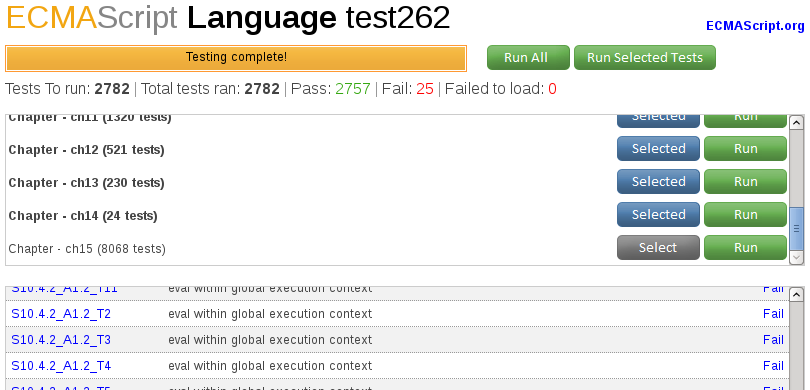
\includegraphics[width = 4cm]{images/test262_small.png}} ;
    \node [below = 0pt of tests] {Test suites} ;

    % \draw<2-> [->, thick] (tests) to node (testing) {} (interp) ;

    % \node<3> [locnode plum, left of = testing] (bisect) {\textsc{Bisect}} ;

    % \draw<3> [->, thick, DarkPlum] (bisect) -- (testing) ;

    % \draw<2-> [<->, thick] (ocaml) -- (jsref) ;

    \draw [<->, thick, Plum] (tests) --
        node [sloped, above, fill = white] {Running tests}
        (jsref) ;

    \node<1> [above of = semlim, locnode brown] (jscert) {\jscert} ;
    \node<2> [dashed, above of = semlim, locnode brown] (jscert) {\jscert} ;

    \draw<1> [->, thick, DarkPlum] (jsref) -- node [above] {Correctness} (jscert) ;
    \draw<2> [->, dashed, thick, DarkPlum] (jsref) -- node [above] {Correctness} (jscert) ;

%   \node [above of = jscert, node distance = 1cm] (next) {} ;
%   \draw [dashed, ->] (jscert) -- (next) ;
%   \node [above of = jscert, left = 3mm, node distance = 1cm] (nextl) {} ;
%   \draw [dashed, ->] (jscert) -- (nextl) ;
%   \node [above of = jscert, right = 3mm, node distance = 1cm] (nextr) {} ;
%   \draw [dashed, ->] (jscert) -- (nextr) ;

    \node [locnode orange, below of = semlim, node distance = 32mm] (ecma) {
\includegraphics[width = 15mm]{images/ecmastandard.png}} ;

    \draw<1> [<->, thick, Plum] (ecma) --
        node [sloped, above, fill = white] {Step / rule}
        node [sloped, below, fill = white] {correspondence} (jscert) ;
    \draw<2> [<->, dashed, thick, Plum] (ecma) --
        node [sloped, above, fill = white] {Step / rule}
        node [sloped, below, fill = white] {correspondence} (jscert) ;

    \draw<2> [<->, thick, Plum] (ecma) --
        node [sloped, above, fill = white] {Step}
        node [sloped, below, fill = white] {correspondence} (jsref) ;

%    \node [right of = ecma, below, node distance = 3cm] {\texttt{jscert.org}} ;

\end{centertikz}

\end{frame}

\begin{frame}
    \frametitle{A Stratified Approach}

    \begin{widemargin}
    \begin{centertikz}
        \node [locnode] (GNUR) {\R{} reference interpreter} ;
        \node [right = 1cm of GNUR] {Lots of code for memory handling} ;

        \node [above = 1cm of GNUR, xshift = -3cm] (linel) {} ;
        \node [above = 1cm of GNUR, xshift = 8cm] (liner) {} ;
        \draw [dashed] (linel) -- (liner) ;
        \node [below = 0mm of liner, xshift = -1cm] {\Cn{}} ;
        \node [above = 0mm of liner, xshift = -1cm] {\Coq{}} ;

        \node [locnode, above = 2cm of GNUR] (proveR) {\Coq{} monadic interpreter} ;
        \node [right = 1cm of proveR] {Close to the \Cn{}} ;

        \node [locnode, dashed, above = 2cm of proveR] (semantics) {Rule-based semantics} ;
        \node [right = 1cm of semantics] {As usable as possible} ;

        \draw<2> [<->, dashed, DarkPlum, thick] (proveR) -- node [right] {\Coq{} proof} (semantics) ;
        \draw<2> [<->, DarkPlum, thick] (GNUR) to [bend right] node [right, pos = .3] {Eyeball closeness} (proveR) ;
        \draw<2> [<->, DarkPlum, thick] (GNUR) to [bend left] node [left, pos = .7] {Testing} (proveR) ;
    \end{centertikz}
    \end{widemargin}

\end{frame}


\section{Eyeball Closeness}

\sectionframe**{Eyeball Closeness}{
    \begin{itemize}
        \item \Cn{} is imperative, pointer-based;
        \item \Coq{} is purely functional, value-based;
        \item The translation is based on a monad \(\mathrm{state}+\mathrm{error}\).
    \end{itemize}
}

\begin{frame}[fragile]
    \frametitle{Eyeball Closeness: Enumeration}

    \begin{minipage}{.45\textwidth}
        \Cn{} code

\begin{ccode}
typedef enum {
    NILSXP  = 0,
    SYMSXP  = 1,
    LISTSXP = 2,
    CLOSXP  = 3,
    ENVSXP  = 4,
    PROMSXP = 5,
    /* ... */
} SEXPTYPE;
\end{ccode}

    \end{minipage}
    \qquad
    \begin{minipage}{.45\textwidth}
        \Coq{} code

\begin{coqcode}
Inductive SExpType :=
  | NilSxp
  | SymSxp
  | ListSxp
  | CloSxp
  | EnvSxp
  | PromSxp
  (* ... *)
  .
\end{coqcode}

    \end{minipage}

    %\begin{itemize}
    %    \item Enumerations are actually more natural in \Coq{} than in \Cn{}.
    %\end{itemize}

\end{frame}

\begin{frame}[fragile]
    \frametitle{Eyeball Closeness: Records}

    \begin{minipage}{.45\textwidth}
        \Cn{} code

\begin{ccode}
struct sxpinfo_struct {
  SEXPTYPE type      :  5;
  unsigned int obj   :  1;
  unsigned int named :  2;
  unsigned int gp    : 16;
  unsigned int mark  :  1;
  unsigned int debug :  1;
  unsigned int trace :  1;
  unsigned int spare :  1;
  unsigned int gcgen :  1;
  unsigned int gccls :  3;
};
/* Total: 32 bits */
\end{ccode}

    \end{minipage}
    \qquad
    \begin{minipage}{.45\textwidth}
        \Coq{} code

\begin{coqcode}
Inductive named_field :=
  | named_temporary
  | named_unique
  | named_plural
  .

Record SxpInfo :=
  make_SxpInfo {
    type : SExpType ;
    obj : bool ;
    named : named_field ;
    gp : nbits 16
  }.
\end{coqcode}

    \end{minipage}

    %\begin{itemize}
    %    \item We recognise some formalisation choices,
    %        but still close enough.
    %\end{itemize}

\end{frame}

\begin{frame}[fragile]
    \frametitle{Eyeball Closeness: Unions}

    \begin{changemargin}{-5mm}{-5mm}
\begin{minipage}{.75\textwidth}
\begin{ccode}
union {
    struct primsxp_struct primsxp;
    struct symsxp_struct symsxp;
    struct listsxp_struct listsxp;
    /* ... */
};
\end{ccode}
\end{minipage}
    \begin{minipage}{.3\textwidth}
    {\Cn{} code}

    \begin{itemize}
        \item Accesses are unsafe.
    \end{itemize}
    \end{minipage}

\begin{minipage}{.75\textwidth}
\begin{coqcode}
Inductive SExpRec_union :=
  | primSxp : PrimSxp_struct -> SExpRec_union
  | symSxp : SymSxp_struct -> SExpRec_union
  | listSxp : ListSxp_struct -> SExpRec_union
  (* ... *)
  .
\end{coqcode}
\end{minipage}
    \begin{minipage}{.3\textwidth}
    {\Coq{} code}

    \begin{itemize}
        \item Accesses must be guarded.
    \end{itemize}
    \end{minipage}
\end{changemargin}

    %\begin{itemize}
    %    \item Large conceptual differences,
    %        but still an eyeball closeness in the definitions.
    %\end{itemize}

\end{frame}

\begin{frame}[fragile]
    \frametitle{Eyeball Closeness: Reading Pointers}

    \vspace{-1mm}
    \begin{changemargin}{-5mm}{-5mm}
\begin{minipage}{.53\textwidth}
    {\Cn{} code}
\begin{ccode}
symsxp_struct p_sym = p->symsxp;
/* ... */
\end{ccode}
\end{minipage}\hspace{6mm}%
\begin{minipage}{.50\textwidth}
    {\Coq{} code}
\begin{coqcode}
read%sym p_sym := p using S in
(* ... *)
\end{coqcode}
\end{minipage}
    \vspace{-1mm}

\begin{coqcode}
Inductive result (T : Type) :=
  | result_success : state -> T -> result T
  | result_error : result T.
\end{coqcode}

\begin{coqcode}
Notation "'read%sym' p_sym ':=' p 'using' S 'in' cont" :=
  (match read S p with
   | Some p_ =>
     match p_ with
     | symSxp p_sym => cont
     | _ => result_error
     end
   | None => result_error
   end).
\end{coqcode}
    \end{changemargin}

\end{frame}

\begin{frame}[fragile]
    \frametitle{Eyeball Closeness: \Cn{} Code}

\begin{changemargin}{-5mm}{-5mm}
\begin{ccode}
EXP* applyClosure (EXP* op, EXP* arglist, EXP* rho){

  EXP* formals, actuals, savedrho, newrho, res;

  if (rho->type != ENVSXP)
    error ("'rho' must be an environment.");

  formals = op->clo.formals;
  savedrho = op->clo.env;

  PROTECT (actuals = matchArgs (formals, arglist));

  /* ... */

  return res;
}
\end{ccode}
\end{changemargin}

\end{frame}

\begin{frame}[fragile]
    \frametitle{Eyeball Closeness: \Coq{} Code}

\begin{changemargin}{-5mm}{-5mm}
\begin{coqcode}
Definition applyClosure (S : state) (op arglist rho : EXP_pointer)
    : result EXP_pointer :=

  read%defined rho_ := rho using S in
  ifb type rho_ <> EnvSxp then
    result_error S "'rho' must be an environment."
  else
    read%clo op_clo := op using S in
    let formals := clo_formals op_clo in
    let savedrho := clo_env op_clo in

    let%success actuals := matchArgs S formals arglist using S in

    (* ... *)

    result_success S res.
\end{coqcode}
\end{changemargin}

\end{frame}

\sectionframe{\R{} Features}

\begin{frame}[fragile]
    \frametitle{\R{} Core}

\begin{ccode}
FUNTAB R_FunTab[] = {
  {"if",        do_if,        2},
  {"while",     do_while,     2},
  {"break",     do_break,     0},
  {"return",    do_return,    1},
  {"function",  do_function,  -1},
  {"<-",        do_set,       2},
  {"(",         do_paren,     1},
  /* ... */
  {"+",         do_arith1,    2},
  {"-",         do_arith2,    2},
  {"*",         do_arith3,    2},
  {"/",         do_arith4,    2},
  /* ... */
  {"cos",       do_math20,    1},
  {"sin",       do_math21,    1},
  {"tan",       do_math22,    1},
  /* ... */ }
\end{ccode}

    \begin{overlayarea}{\textwidth}{0cm}
        \only<2>{
            \vspace{-8cm}
            \parbox[t]{0pt}{
                \centering{}~\hspace{-1cm}%
                \tikz \fill[white] (0, 0) rectangle (12, 6) ;
            }%
            \vspace{-6cm} % WTF KNUTH
            \begin{block}{The core is what is needed to call these functions.}
                \begin{itemize}
                    \item The core is small;
                    \item The formalisation is easily extendable.
                \end{itemize}
            \end{block}
            \begin{block}{Content of the core}
                \begin{itemize}
                    \item Expression evaluation;
                    \item Function calls;
                    \item Environments, delayed evaluation (promises);
                    \item Initialisation of the global state.
                \end{itemize}
            \end{block}
        }
    \end{overlayarea}

% C.
% Separation between core and non-core.

\end{frame}

\begin{frame}
    \frametitle{Future}

    \begin{block}{The current formalisation is modular}
        \begin{itemize}
            \item It is easy to add features.
            \item We can implement specific features and certify their implementations.
        \end{itemize}
    \end{block}

    \pause

    \begin{block}{Providing trust}
        \begin{itemize}
            \item Test the formalisation…
            \item …or certify it (CompCert’s semantics, Formalin, etc.).
        \end{itemize}
    \end{block}

    \pause

    \begin{block}{Building proofs}
        \vspace{-4mm}
        \[
            \left.
                \mbox{\begin{minipage}{5cm}
                    \begin{itemize}
                        \item Building a rule-based formalisation;
                        \item A more functional interpreter.
                    \end{itemize}
                \end{minipage}}
            \right\} \mbox{\parbox{5cm}{What is the best to build large proofs of programs?}}
        \]
    \end{block}

    % To be useful for Coq users
    % To be useful for the R community (RExplain?).

\end{frame}

\begin{frame}[fragile]
    \frametitle{Proof that \(1 + 1\) reduces to \(2\) in \jscert{}}

\begin{coqcode}[fontsize = \tiny]
Lemma one_plus_one_exec : forall S C,
  red_expr S C one_plus_one (out_ter S (prim_number two)).
Proof.
  intros. unfold one_plus_one.
  eapply red_expr_binary_op.
   constructor.
   eapply red_spec_expr_get_value.
    eapply red_expr_literal. reflexivity.
   eapply red_spec_expr_get_value_1.
   eapply red_spec_ref_get_value_value.
  eapply red_expr_binary_op_1.
   eapply red_spec_expr_get_value.
    eapply red_expr_literal. reflexivity.
   eapply red_spec_expr_get_value_1.
   eapply red_spec_ref_get_value_value.
  eapply red_expr_binary_op_2.
  eapply red_expr_binary_op_add.
   eapply red_spec_convert_twice.
    eapply red_spec_to_primitive_pref_prim.
   eapply red_spec_convert_twice_1.
    eapply red_spec_to_primitive_pref_prim.
   eapply red_spec_convert_twice_2.
  eapply red_expr_binary_op_add_1_number.
   simpl. intros [A|A]; inversion A.
   eapply red_spec_convert_twice.
    eapply red_spec_to_number_prim. reflexivity.
   eapply red_spec_convert_twice_1.
    eapply red_spec_to_number_prim. reflexivity.
   eapply red_spec_convert_twice_2.
  eapply red_expr_puremath_op_1. reflexivity.
Qed.
\end{coqcode}

\end{frame}

\begin{frame}[fragile]
    \frametitle{RExplain}

   %\begin{block}{In practise, JavaScript people read JSRef, not \jscert{}}
   %    \begin{itemize}
   %        \item An executable \R{} interpreter would be easier to read than a rule-based semantics;
   %        \item Some want to specify \R{}, we may propose a solution.
   %    \end{itemize}
   %\end{block}

    \begin{widemargin}
    \begin{centertikz}
        \node [locnode] (imp) {\begin{minipage}{52mm}
            Imperative interpreter
\begin{camlcode}[linenos = false]
let%success res = f args in
read%clo res_clo = res in
\end{camlcode}
            \end{minipage}} ;
        \node [locnode, right = 5mm of imp] (func) {\begin{minipage}{65mm}
            Functionnal interpreter
\begin{camlcode}[linenos = false]
let%success res = f S args using S in
read%clo res_clo = res using S in
\end{camlcode}
            \end{minipage}} ;
        \node [locnode, below = 5mm of imp, xshift = 4cm] (spec) {\begin{minipage}{10cm}
            ECMA-style specification
            \begin{enumerate}
                \item Let \mintedinlinespacebug\camlinline{res} be the result
                    of calling \mintedinlinespacebug\camlinline{f} with argument
                    \mintedinlinespacebug\camlinline{args};
                \item At this stage, \mintedinlinespacebug\camlinline{res} should
                    be a closure.
            \end{enumerate}
            \end{minipage}} ;
        \node [locnode, below = 5mm of spec] (rbs) {\begin{minipage}{10cm}
            Rule-based semantics
\begin{coqcode}[linenos = false, fontsize = \tiny]
| run_1 : forall S args o1 o2,
  run S (f args) o1 -> run S (term_1 o1) o2 -> run S (term o1) o2
| run_2 : forall S res_clo o,
  is_closure S res res_clo -> run S (term_2 res_clo) o -> run S (term_1 (out S res)) o
\end{coqcode}
            \end{minipage}} ;
        \draw [->, thick] (imp) to (func) ;
        \draw [->, thick] (imp.-150) to [bend right = 25] (rbs) ;
        \draw [->, thick] (imp) to (spec) ;
    \end{centertikz}
    \end{widemargin}

    \url{https://github.com/jscert/jsexplain}

\end{frame}

\begin{frame}
    \frametitle{Thank you for listening!}

    \vspace{-1mm}
    \begin{block}{The current formalisation is modular}
        \begin{itemize}
            \item It is easy to add features.
            \item We can implement specific features and certify their implementations.
        \end{itemize}
    \end{block}

    \begin{block}{Providing trust}
        \begin{itemize}
            \item Test the formalisation…
            \item …or certify it (CompCert’s semantics, Formalin, etc.).
        \end{itemize}
    \end{block}

    \begin{block}{Building proofs}
        \vspace{-4mm}
        \[
            \left.
                \mbox{\begin{minipage}{5cm}
                    \begin{itemize}
                        \item Building a rule-based formalisation;
                        \item A more functional interpreter.
                    \end{itemize}
                \end{minipage}}
            \right\} \mbox{\parbox{5cm}{What is the best to build large proofs of programs?}}
        \]
    \end{block}

    \url{https://github.com/Mbodin/proveR}

\end{frame}

\frame{\tableofcontents}

\sectionframe*{Bonuses}

\newcommand\questiontoc{
    %\begin{multicols}{2}
    \begin{enumerate}
        \item \hyperlink{frame:jscert}{\jscert{}};
        \item \hyperlink{frame:imperative:functional}{Representing imperativity in a functional setting};
        \item \hyperlink{frame:semantics:coq}{Semantics in \coqn{}};
        \item \hyperlink{frame:semantic:sizes}{Semantic sizes};
        \item \hyperlink{frame:other:subtleties}{Other Subtleties of \R{}};
        \item \hyperlink{frame:reading:pointers}{Reading pointers};
        \item \hyperlink{frame:parser}{Parsing \R{}};
        \item \hyperlink{frame:full:monad}{The full state+error monad};
        \item \hyperlink{frame:input:output}{Inputs and outputs}.
    \end{enumerate}
    %\end{multicols}
}

\frame{\questiontoc}

\begin{frame}
    \label{frame:jscert}
    \frametitle{The \jscert{} Project
        \hfill\hfill\hfill
        \raisebox{-10mm}[0pt][0pt]{
            
\includegraphics[width = 15mm]{images/jscert.png} ;
        }}

\begin{centertikz}[node distance = 1.5cm]

    \node (realworldleft) {};
    \node [right of = realworldleft, node distance = 11.5cm] (realworldright) {} ;

    \node [right of = realworldleft, node distance = 1.5cm] (semlim) {} ;
    \node [left of = realworldright, node distance = 4cm] (testlim) {} ;

    \draw [dashed] (realworldleft) to node[above, pos = 0.9] {\coqn{} definitions} node [below, pos = 0.9] {Industrial world} (realworldright) ;

    % \node<2-> [below of = testlim, locnode] (ocaml) {\parbox{1.5cm}{\centering\camln{}\\extraction}} ;
    % \node<2-> [right of = ocaml, node distance = 2cm, locnode] (parser) {Parser} ;

\begin{pgfonlayer}{background}
    % \node<2-> [fit = (ocaml) (parser), locnode yellow] (interp) {} ;
\end{pgfonlayer}

    \node [above of = testlim, locnode brown] (jsref) {\jsref} ;
    \node [above = 0pt of jsref] {\(\sim{}3,000\)~lines of code} ;

    \node [locnode blue, below of = jsref, node distance = 45mm] (tests) {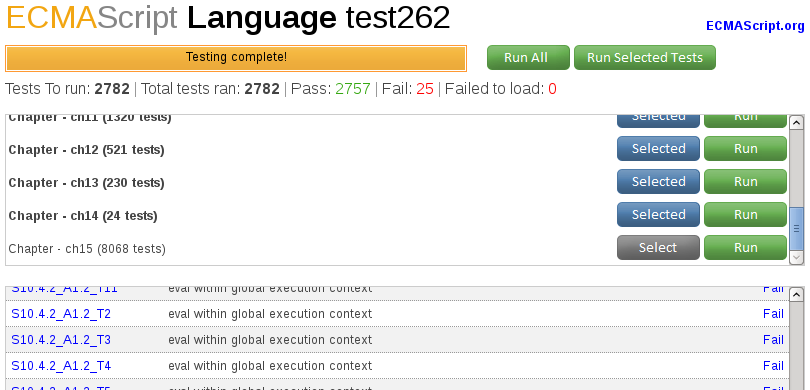
\includegraphics[width = 4cm]{images/test262_small.png}} ;
    \node [below = 0pt of tests] {\(5,126\)~tests passed} ; % out of~\(11,725\)} ;

    % \draw<2-> [->, thick] (tests) to node (testing) {} (interp) ;

    % \node<3> [locnode plum, left of = testing] (bisect) {\textsc{Bisect}} ;

    % \draw<3> [->, thick, DarkPlum] (bisect) -- (testing) ;

    % \draw<2-> [<->, thick] (ocaml) -- (jsref) ;

    \draw [<->, thick, Plum] (tests) --
        node [sloped, above, fill = white] {Running tests}
        (jsref) ;

    \node [above of = semlim, locnode brown] (jscert) {\jscert} ;
    \node [above = 0pt of jscert] {\(\sim{}900\)~rules} ;

    \draw [->, thick, DarkPlum] (jsref) -- node [above] {Correctness}
            node [below, Aluminium6] {\(\sim{}6,000\)~lines of proof} (jscert) ;

%   \node [above of = jscert, node distance = 1cm] (next) {} ;
%   \draw [dashed, ->] (jscert) -- (next) ;
%   \node [above of = jscert, left = 3mm, node distance = 1cm] (nextl) {} ;
%   \draw [dashed, ->] (jscert) -- (nextl) ;
%   \node [above of = jscert, right = 3mm, node distance = 1cm] (nextr) {} ;
%   \draw [dashed, ->] (jscert) -- (nextr) ;

    \node [locnode orange, below of = semlim, node distance = 32mm] (ecma) {
\includegraphics[width = 15mm]{images/ecmastandard.png}} ;
    \node [below = 0pt of ecma] {\(\sim{}900\)~steps} ;

    \draw [<->, thick, Plum] (ecma) --
        node [sloped, above, fill = white] {Step / rule}
        node [sloped, below, fill = white] {correspondence} (jscert) ;


%    \node [right of = ecma, below, node distance = 3cm] {\texttt{jscert.org}} ;

\end{centertikz}

\end{frame}

\frame{\questiontoc}

\begin{frame}[fragile]
    \label{frame:imperative:functional}
    \frametitle{How to Represent Imperative Features in a Functional Setting}

    \begin{itemize}
        \item Structures like maps are easy to implement;
        \item We can represent every element of the state of a program \\
            (memory, outputs, etc.) in a data-structure;
        \item We have to pass this structure along the program.
    \end{itemize}

    \begin{block}{Enter the monad}
\begin{camlcode}
if_success (run s1 p) (fun s2 =>
  let s3 = write s2 x v in
  if_success (run s3 p') (fun s4 =>
    return_success s4))
\end{camlcode}
    \end{block}

\end{frame}

\frame{\questiontoc}

\begin{frame}[fragile]
    \label{frame:semantics:coq}
    \frametitle{Formalisation of Semantics in \coqn{}}

\begin{coqcode}
Inductive semantics : state -> prog -> state -> Prop ->

  | semantics_skip : forall s p, semantics s p s

  | semantics_seq : forall s1 s2 s3 p1 p2,
    semantics s1 p1 s2 ->
    semantics s2 p2 s3 ->
    semantics s1 (seq p1 p2) s3

  | semantics_asgn : forall s x v,
    semantics s (asgn x v) (write s x v)
  .
\end{coqcode}

\end{frame}

\begin{frame}
    \frametitle{Sequence in \jscert{} (Paper Version)}

    \begin{overlayarea}{\textwidth}{3cm}
    \begin{block}{“\mintedinlinespacebug\jsinline|s1 ; s2|” is evaluated as follows.}
\begin{enumerate}
    \item Let~\(o_1\) be the result of evaluating~\mintedinlinespacebug\jsinline|s1|.
    \item If~\(o_1\) is an exception, return~\(o_1\).
    \item Let~\(o_2\) be the result of evaluating~\mintedinlinespacebug\jsinline|s2|.
    \only<1>{
        \item If an exception~\(\mathit{V}\) was thrown, return \(\mpar{\jstthrow{}, \mathit{V}, \mathit{empty}}\). % where \(\mathit{V}\)~is the exception.
            % (Execution now proceeds as if no exception were thrown.)
        \item If~\(\mathit{o_2}.\mathit{value}\) is empty, let~\(\mathit{V} = \mathit{o_1}.\mathit{value}\),
            otherwise let~\(\mathit{V} = \mathit{o_2}.\mathit{value}\).
        \item Return \(\mpar{\mathit{o_2}.\mathit{type}, \mathit{V}, \mathit{o_2}.\mathit{target}}\).
    }
\end{enumerate}
    \end{block}
    \end{overlayarea}

    \visible<3>{
\begin{mathpar}
    \inferrule[seq-1\(\fund{s_1}{s_2}\)]
    { S, C, s_1 \evalr o_1 \\ o_1, \seqx{s_2} \evalr o }
    { S, C, \seq{s_1}{s_2} \evalr o }
    \and
    \inferrule[seq-2\(\funu{s_2}\)]
    { }
    { o_1, \seqx{s_2} \evalr o_1 }
    \quad { \abort{o_1} }
    \and
    \inferrule[seq-3\(\funu{s_2}\)]
    { o_1, s_2 \evalr o_2 \\ o_1, o_2, \seqxx{} \evalr o }
    { o_1, \seqx{s_2} \evalr o }
    \quad { \neg\abort{o_1} }
    \and
    \ldots
\end{mathpar}
}

\end{frame}

\begin{frame}[fragile]
    \label{frame:seq:jscert}
    \frametitle{Sequence in \jscert{}}

%  | red_stat_abort : forall S C extt o,
%    out_of_ext_stat extt = Some o →
%    abort o ->
%    ~ abort_intercepted_stat extt →
%    red_stat S C extt o

\begin{changemargin}{-5.5mm}{-9mm}
\begin{coqcode}
Inductive red_stat : state → scope → stat → out → Prop :=

| red_stat_seq_1 : forall S C s1 s2 o1 o,
  red_stat S C s1 o1 →
  red_stat S C (seq_1 s2 o1) o →@\anchor{seq1}{}@
  red_stat S C (seq s1 s2) o

| red_stat_seq_2 : forall S C s2 o1,
  abort o1 →@\anchor{seq2}{}@
  red_stat S C (seq_1 s2 o1) o1

| red_stat_seq_3 : forall S0 S C s2 o2 o,
  red_stat S C s2 o2 →@\anchor{seq3}{}@
  red_stat S C (seq_2 o2) o →
  red_stat S0 C (seq_1 s2 (out_ter S)) o

(* ... *).
\end{coqcode}
\end{changemargin}
\begin{innertikz}[overlay, remember picture]
    \def\distshift{35mm} % WTF: This looks like a TikZ bug: nodes appear this distance below their supposed location…
    \node [right = 25mm of seq1, yshift = \distshift, scale = .8] {\(
        \inferrule[seq-\raisebox{.6ex}{\bsphere{1}}\(\fund{s_1}{s_2}\)]
        { S, C, s_1 \evalr o_1 \\ o_1, \seqx{s_2} \evalr o }
        { S, C, \seq{s_1}{s_2} \evalr o }
    \)} ;
    \node [right = 64mm of seq2, yshift = \distshift, scale = .8] {\(
        \inferrule[seq-\raisebox{.6ex}{\bsphere{2}}\(\funu{s_2}\)]
        { }
        { o_1, \seqx{s_2} \evalr o_1 }
        \quad { \abort{o_1} }
    \)} ;
    \node [right = 34mm of seq3, yshift = \distshift, scale = .7] {\(
        \inferrule[seq-\raisebox{.55ex}{\bsphere{3}}\(\funu{s_2}\)]
        { o_1, s_2 \evalr o_2 \\ o_1, o_2, \seqxx{} \evalr o }
        { o_1, \seqx{s_2} \evalr o }
        \quad { \neg\abort{o_1} }
    \)} ;
\end{innertikz}

\end{frame}

\frame{\questiontoc}

\begin{frame}
    \label{frame:semantic:sizes}
    \frametitle{Semantic Sizes}

    \begin{centertikz}
        \node (lambda) {\(\lambda\)-calculus} ;
        \node [right = 5mm of lambda] (ml) {CoreML} ;
        \node [right = 5mm of ml] (compcert) {\CompCert{} \Cn{}} ;
        \node [right = 5mm of compcert] (jscert) {\jscert{}} ;

        \draw [DarkPlum, fill = LightPlum] ($(lambda.north) + (-.5, .1)$) rectangle ++ (1, .003) ;
        \node [above = 1mm of lambda] {\(3\)~rules} ; % 5 in pretty-big-step.

        \draw [DarkPlum, fill = LightPlum] ($(ml.north) + (-.5, .1)$) rectangle ++ (1, .25) ;
        \node [above = 3mm of ml] {\(\sim{}50\)~rules} ; % 61 in pretty-big-step.

        \draw [DarkPlum, fill = LightPlum] ($(compcert.north) + (-.5, .1)$) rectangle ++ (1, 1) ;
        \node [above = 11mm of compcert] {\(\sim{}200\)~rules} ; % 110 in big step + 77 in denotational.
        % Source: http://compcert.inria.fr/doc/html/Csem.html and http://compcert.inria.fr/doc/html/Cop.html

        \draw [DarkPlum, fill = LightPlum] ($(jscert.north) + (-.5, .1)$) rectangle ++ (1, 4.5) ;
        \node [above = 46mm of jscert] {\(\sim{}900\)~rules} ; % ~900 in pretty-big-step.

%        \draw [thick, dashed, ->] (compcert) to [bend right] ($(compcert) + (-1, -1)$) ;

    \end{centertikz}
%    \vspace{-5mm}

%   \begin{refsection}
%       \nocite{Verasco}
%       \printbibliography{}
%   \end{refsection}

\end{frame}

\frame{\questiontoc}

\begin{frame}[fragile]
    \label{frame:other:subtleties}
    \frametitle{Other Subtleties}

%\begin{onlyenv}<1>
\begin{Rcode}
f <- function (x, y, option, longArgumentName) ...

# All the following calls are equivalent.
f (1, 2, "something", 42)
f (option = "something", 1, 2, 42)
f (opt = "something", long = 42, 1, 2)
\end{Rcode}
%\end{onlyenv}

\begin{overlayarea}{\textwidth}{5cm}
\begin{onlyenv}<2>
\begin{Rcode}
f <- function (abc, ab, de) c (abc, ab, de)

# All the following calls are equivalent.
f (1, 2, 3)
f (de = 3, 1, 2)
f (d = 3, 1, 2)
f (ab = 2, 1, 2)
f (ab = 2, a = 1, 3)

f (a = 3, 1, 2) # Returns an error.
\end{Rcode}
\end{onlyenv}
\end{overlayarea}

\end{frame}

\frame{\questiontoc}

\begin{frame}[fragile]
    \label{frame:reading:pointers}
    \frametitle{Eyeball Closeness: Reading Pointers}

    \begin{changemargin}{-5mm}{-5mm}

\begin{minipage}{.6\textwidth}
    {\Cn{} code}
\begin{ccode}
symsxp_struct p_sym = p->symsxp;
/* ... */
\end{ccode}
\end{minipage}
    \begin{minipage}{.45\textwidth}
    \begin{itemize}
        \item May fail because the pointer \mintedinlinespacebug\cinline|p| is unbound;
        \item May fail because the union \mintedinlinespacebug\cinline|*p| is not a \mintedinlinespacebug\cinline|symsxp|.
    \end{itemize}
    \end{minipage}

\vfill

\parbox{\textwidth}{\onslide<2->{\Coq{} code, \only<2>{first}\only<3>{second}\only<4>{third}\only<5>{fourth} try}}
\begin{minipage}{.5\textwidth}
\begin{overlayarea}{\textwidth}{5cm}
    \begin{onlyenv}<2>
\begin{coqcode}
match read p with
  (* ... *)
end
\end{coqcode}
    \end{onlyenv}
    \begin{onlyenv}<3>
\begin{coqcode}
match read S p with
| Some p_ =>
  match p_ with
  | symSxp p_sym =>
    (* ... *)
  | _ => (* ??? *)
  end
| None => (* ??? *)
end
\end{coqcode}
    \end{onlyenv}
    \begin{onlyenv}<4>
\begin{coqcode}
match read S p with
| Some p_ =>
  match p_ with
  | symSxp p_sym =>
    (* ... *)
  | _ => error
  end
| None => error
end
\end{coqcode}
    \end{onlyenv}
    \begin{onlyenv}<5>
\begin{coqcode}
read%sym p_sym := p using S in
(* ... *)
\end{coqcode}
    \end{onlyenv}
\end{overlayarea}
\end{minipage}\quad
\begin{minipage}{.5\textwidth}
\begin{minipage}{1.2\textwidth}
\begin{overlayarea}{\textwidth}{5cm}
    \begin{onlyenv}<4->
\begin{coqcode}
Inductive result (T : Type) :=
  | success : state -> T -> result T
  | error : result T
  .
\end{coqcode}
    \end{onlyenv}
    \begin{onlyenv}<5->
\begin{coqcode}
Notation "'read%sym' p_sym ':=' p
    'using' S 'in' cont" :=
  (* ... *).
\end{coqcode}
    \end{onlyenv}
\end{overlayarea}
\end{minipage}
\end{minipage}

\end{changemargin}

\end{frame}

\frame{\questiontoc}

\begin{frame}[fragile]
    \label{frame:parser}

\begin{ccodenoescape}
expr:
  | NUM_CONST                   { $$ = $1;  setId( $$, @$); }
  | STR_CONST                   { $$ = $1;  setId( $$, @$); }
  | NULL_CONST                  { $$ = $1;  setId( $$, @$); }          
  | SYMBOL                      { $$ = $1;  setId( $$, @$); }
  | LBRACE exprlist RBRACE
    { $$ = xxexprlist($1,&@1,$2); setId( $$, @$); }
  | LPAR expr_or_assign RPAR
    { $$ = xxparen($1,$2);  setId( $$, @$); }
\end{ccodenoescape}

\begin{camlcode}
expr:
  | c = NUM_CONST                       { c }
  | c = STR_CONST                       { c }
  | c = NULL_CONST                      { c }
  | c = SYMBOL                          { c }
  | b = LBRACE; e = exprlist; RBRACE
    { eatLines := false ; lift2 (only_state xxexprlist) b e }
  | p = LPAR; e = expr_or_assign; RPAR
    { lift2 (no_runs xxparen) p e }
\end{camlcode}

\end{frame}

\frame{\questiontoc}

\begin{frame}[fragile]
    \label{frame:full:monad}
    \frametitle{The Full State+Error Monad}

\begin{coqcode}
Inductive result (A : Type) :=
  | result_success : state -> A -> result A
  | result_error : state -> string -> result A
  | result_longjump : state -> nat -> context_type -> result A
  | result_impossible : state -> string -> result A
  | result_not_implemented : string -> result A
  | result_bottom : state -> result A
  .
\end{coqcode}

\end{frame}

\frame{\questiontoc}

\begin{frame}[fragile]
    \label{frame:input:output}

\begin{coqcode}
Record input := make_input {
    prompt_string : stream string ;
    random_boolean : stream bool
  }.
\end{coqcode}

\begin{coqcode}
Record output := make_output {
    output_string : list string
  }.
\end{coqcode}

\begin{coqcode}
Record state := make_state {
    inputs :> input ;
    outputs :> output ;
    state_memory :> memory ;
    state_context : context
  }.
\end{coqcode}

\end{frame}

\frame{\questiontoc}

\frame{\tableofcontents}

\end{document}

